%\appendix
\chapter{BDT plots}
\label{sec:appBDTplots}


\section{Low mass splittings}
\subsection{Low level features}

\newpage

\begin{figure}[H]
    \centering
    \begin{subfigure}[t!]{0.49\textwidth}
        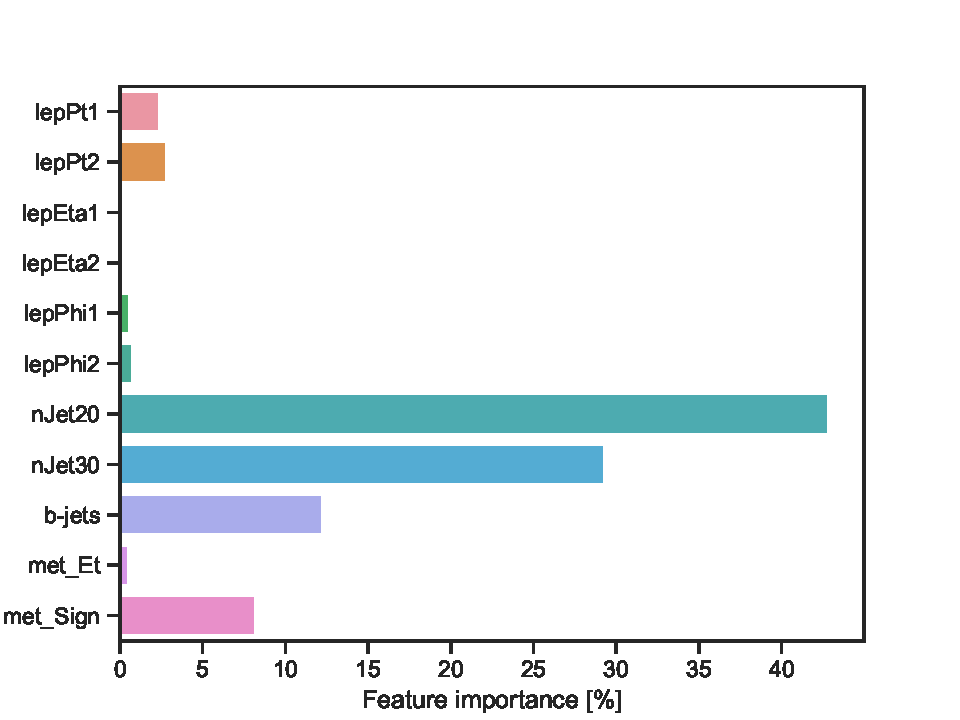
\includegraphics[width = \textwidth]{Figures/SlepSlep/ML/BDT/Low_level/Low/featureImportance.pdf}
        \caption{Direct slepton production.}
        \label{fig:}
    \end{subfigure}
    \begin{subfigure}[t!]{0.49\textwidth}
        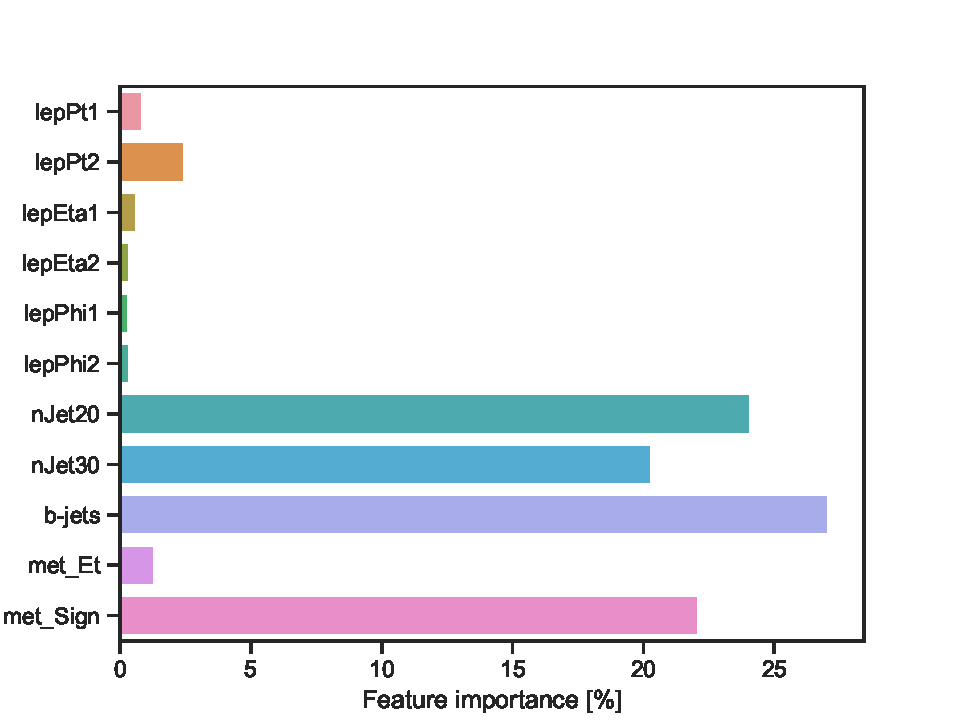
\includegraphics[width = \textwidth]{Figures/SlepSnu/BDT/Low_level/Low/featureImportance.pdf}
        \caption{Chargino production via $\Tilde{l}/\Tilde{\nu}$.}
        \label{fig:}
    \end{subfigure}
    \begin{subfigure}[t!]{0.49\textwidth}
        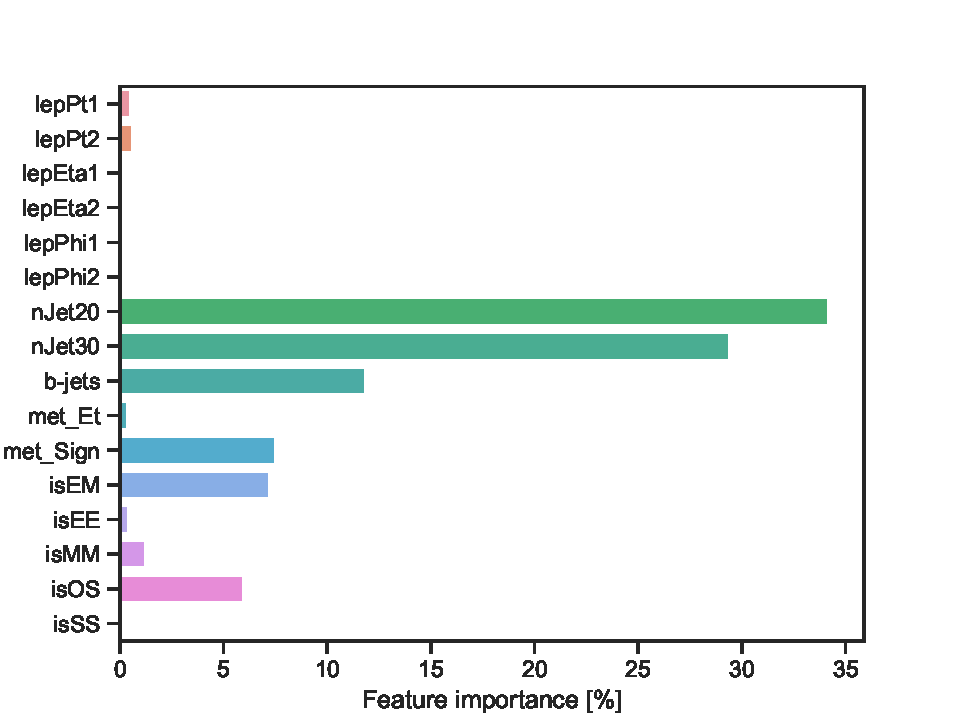
\includegraphics[width = \textwidth]{Figures/WW/BDT/Low_level/Low/featureImportance.pdf}
        \caption{Chargino production via $W^\pm$.}
        \label{fig:}
    \end{subfigure}
    \begin{subfigure}[t!]{0.49\textwidth}
        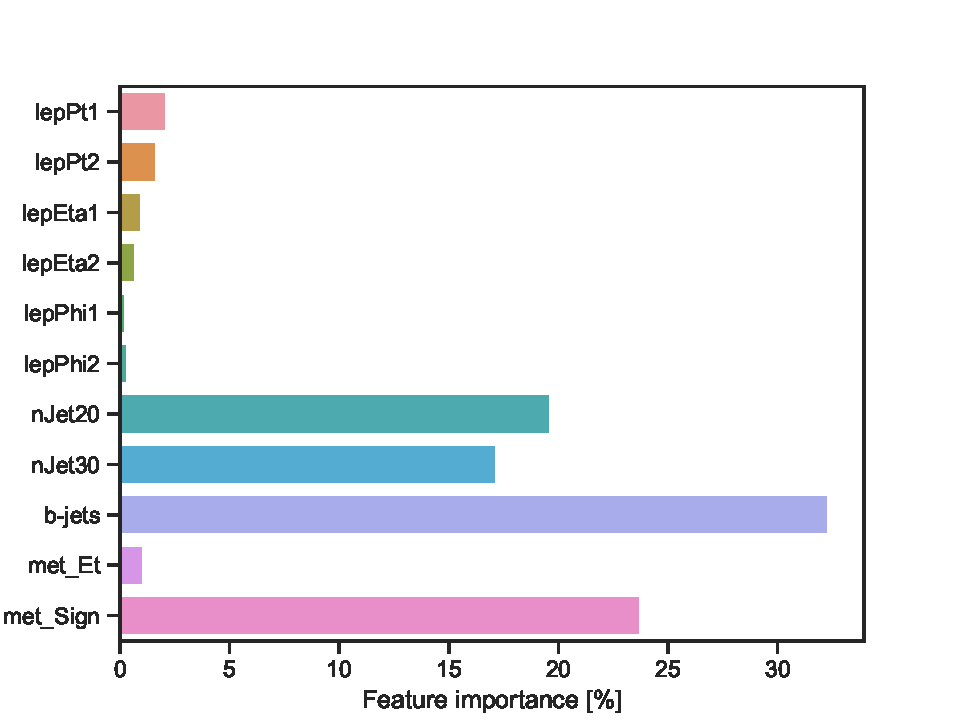
\includegraphics[width = \textwidth]{Figures/Mono_Z/ML/BDT/Low_level/Low/featureImportance.pdf}
        \caption{Mono-Z.}
        \label{fig:}
    \end{subfigure}
    \caption{Feature importance for low mass splittings for all four processes using low level features during training.}
    \label{fig:Non}
\end{figure}


\begin{figure}[H]
    \centering
    \begin{subfigure}[t!]{0.49\textwidth}
        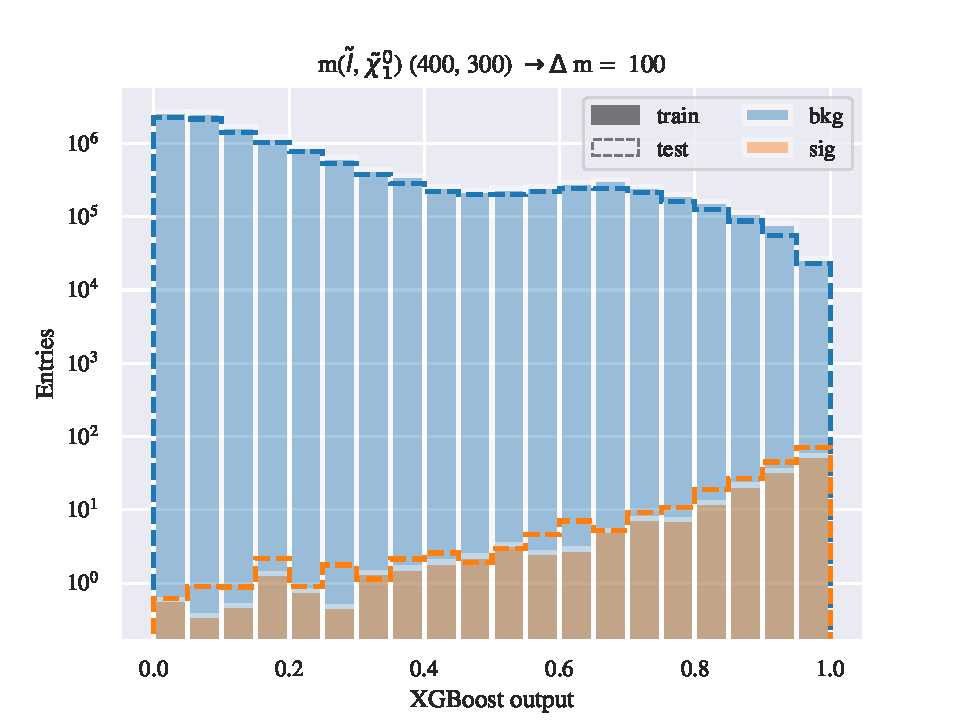
\includegraphics[width = \textwidth]{Figures/SlepSlep/ML/BDT/Low_level/Low/scaled_train_test_395984.pdf}
        \caption{Direct slepton production.}
        \label{fig:}
    \end{subfigure}
    \begin{subfigure}[t!]{0.49\textwidth}
        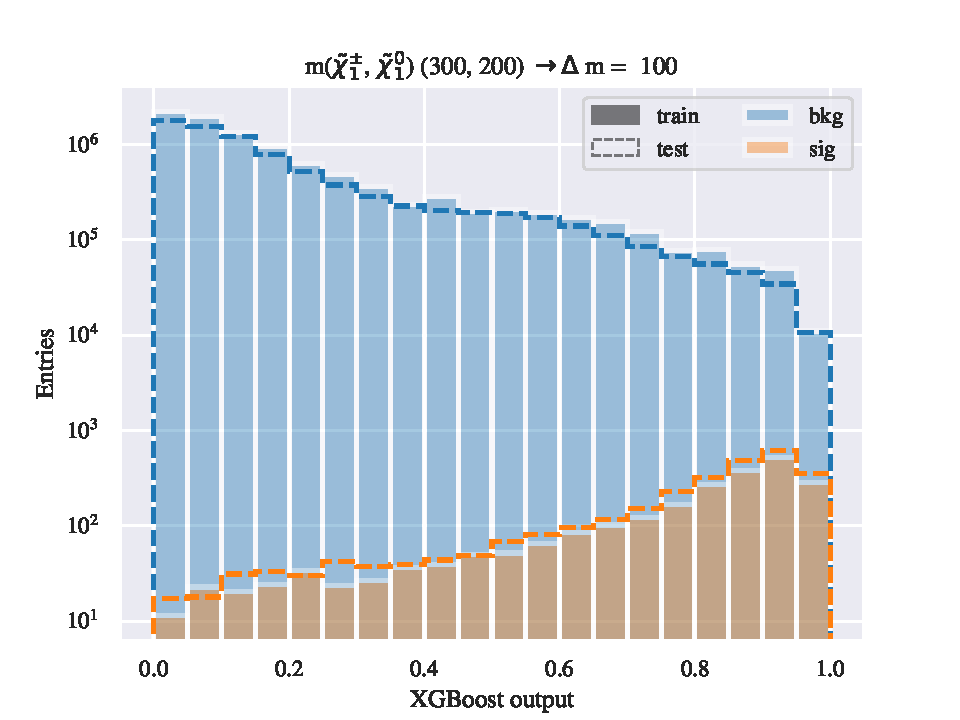
\includegraphics[width = \textwidth]{Figures/SlepSnu/BDT/Low_level/Low/scaled_train_test_397115.pdf}
        \caption{Chargino production via $\Tilde{l}/\Tilde{\nu}$.}
        \label{fig:}
    \end{subfigure}
    \begin{subfigure}[t!]{0.49\textwidth}
        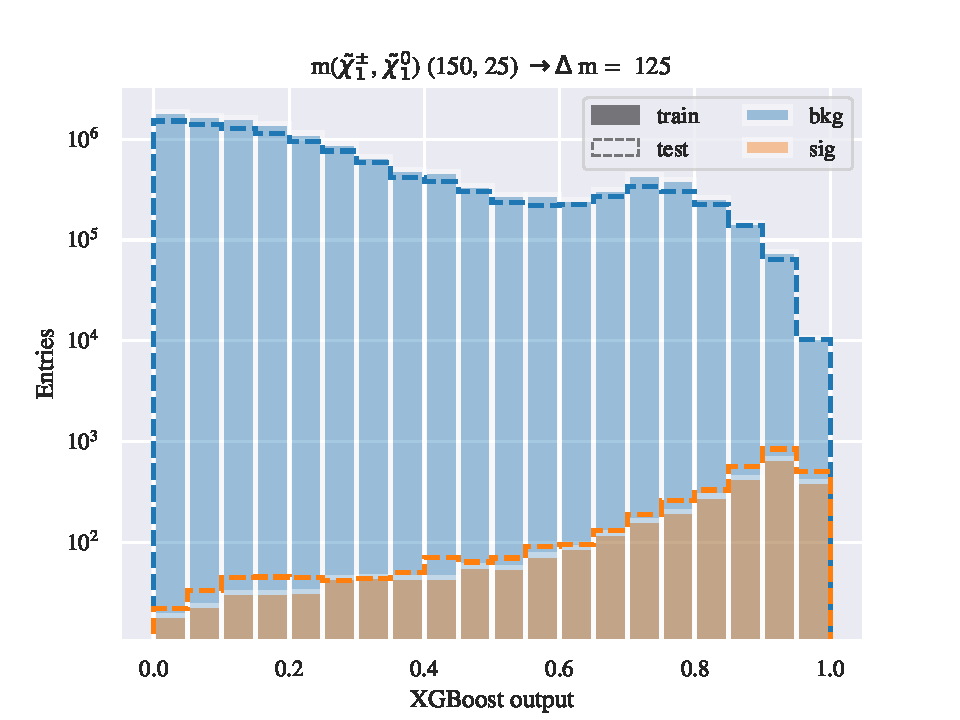
\includegraphics[width = \textwidth]{Figures/WW/BDT/Low_level/Low/scaled_train_test_395268.pdf}
        \caption{Chargino production via $W^\pm$.}
        \label{fig:}
    \end{subfigure}
    \begin{subfigure}[t!]{0.49\textwidth}
        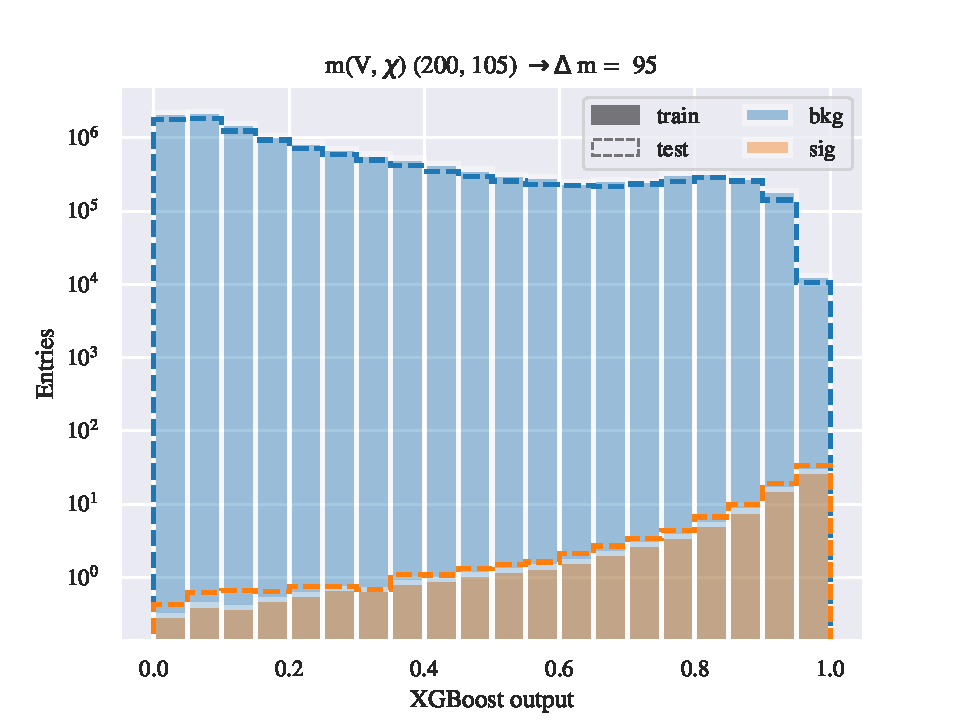
\includegraphics[width = \textwidth]{Figures/Mono_Z/ML/BDT/Low_level/Low/scaled_train_test_310604.pdf}
        \caption{Mono-Z.}
        \label{fig:}
    \end{subfigure}
    \caption{Test vs train for low mass splittings done with the BDT using low level features during training. Here the test set is scaled up to match the number of training events.}
    \label{fig:Non}
\end{figure}



\subsection{High level features}

\begin{figure}[H]
    \centering
    \begin{subfigure}[t!]{0.49\textwidth}
        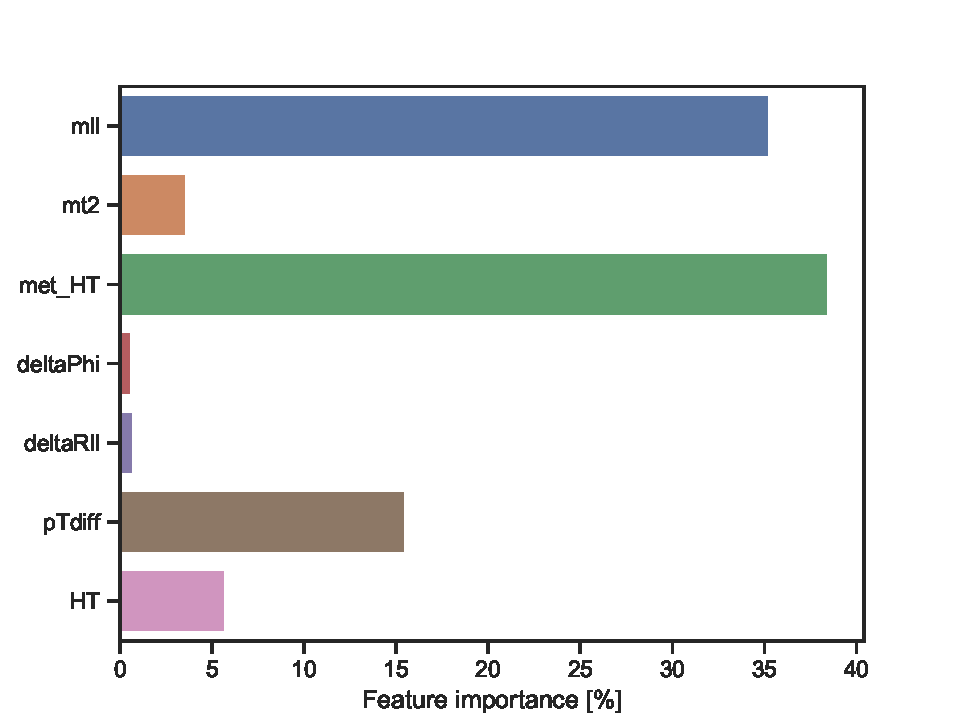
\includegraphics[width = \textwidth]{Figures/SlepSlep/ML/BDT/High_level/Low/featureImportance.pdf}
        \caption{Direct slepton production.}
        \label{fig:featSlepslepLow}
    \end{subfigure}
    \begin{subfigure}[t!]{0.49\textwidth}
        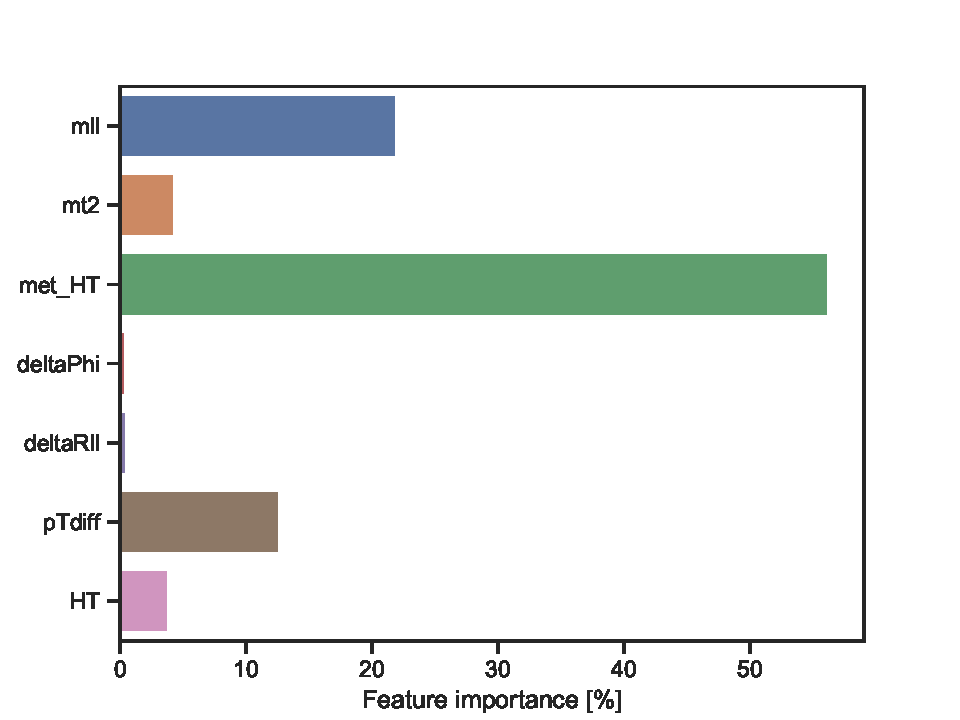
\includegraphics[width = \textwidth]{Figures/SlepSnu/BDT/High_level/Low/featureImportance.pdf}
        \caption{Chargino production via $\Tilde{l}/\Tilde{\nu}$.}
        \label{fig:}
    \end{subfigure}
    \begin{subfigure}[t!]{0.49\textwidth}
        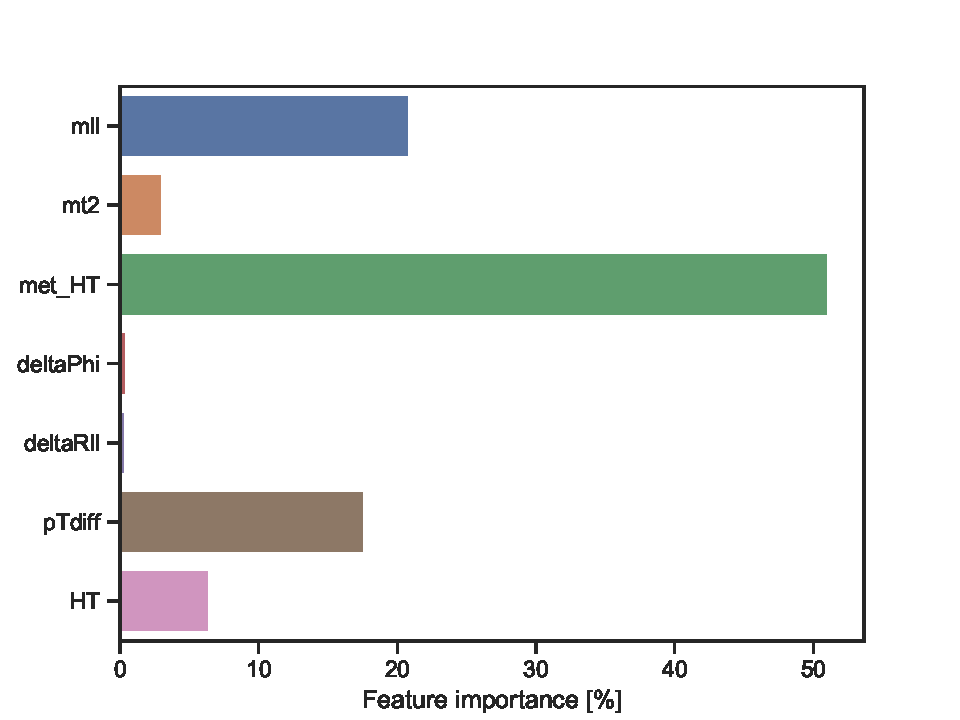
\includegraphics[width = \textwidth]{Figures/WW/BDT/High_level/Low/featureImportance.pdf}
        \caption{Chargino production via $W^\pm$.}
        \label{fig:}
    \end{subfigure}
    \begin{subfigure}[t!]{0.49\textwidth}
        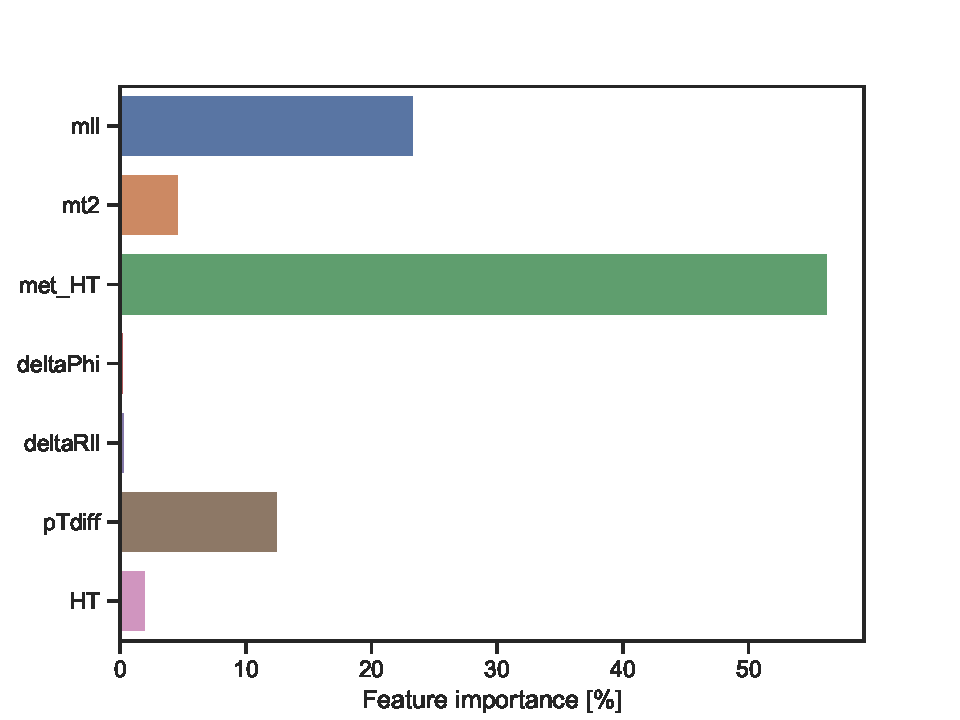
\includegraphics[width = \textwidth]{Figures/Mono_Z/ML/BDT/High_level/Low/featureImportance.pdf}
        \caption{Mono-Z.}
        \label{fig:}
    \end{subfigure}
    \caption{Feature importance for low mass splittings for all four processes using high level features during training.}
    \label{fig:Non}
\end{figure}


\begin{figure}[H]
    \centering
    \begin{subfigure}[t!]{0.49\textwidth}
        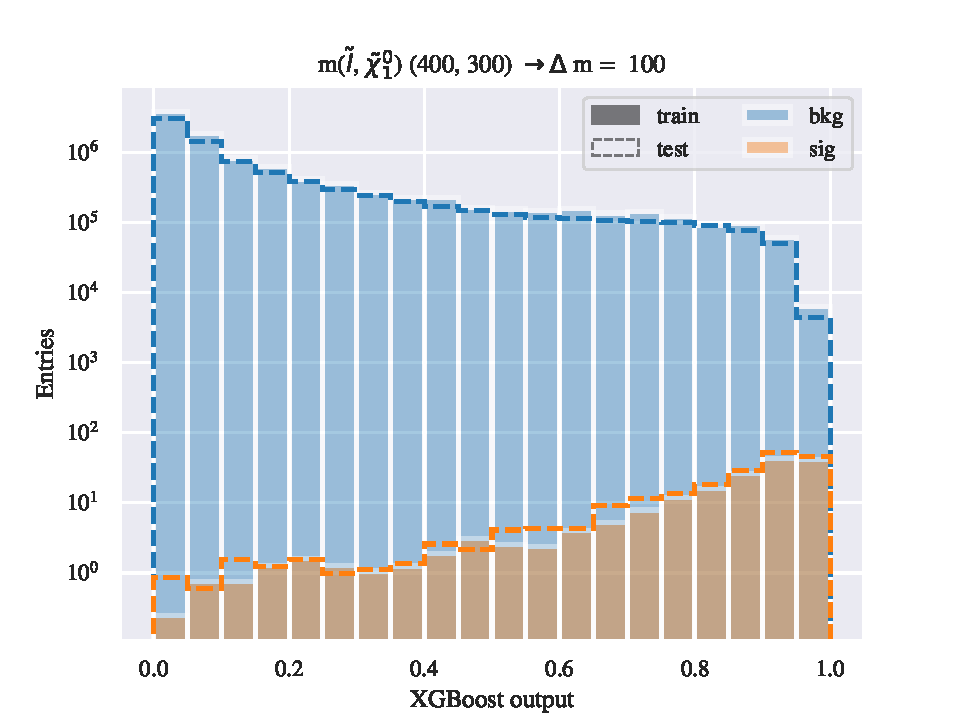
\includegraphics[width = \textwidth]{Figures/SlepSlep/ML/BDT/High_level/Low/scaled_train_test_395984.pdf}
        \caption{Direct slepton production.}
        \label{fig:traintestscaledBDTSlepslepLow}
    \end{subfigure}
    \begin{subfigure}[t!]{0.49\textwidth}
        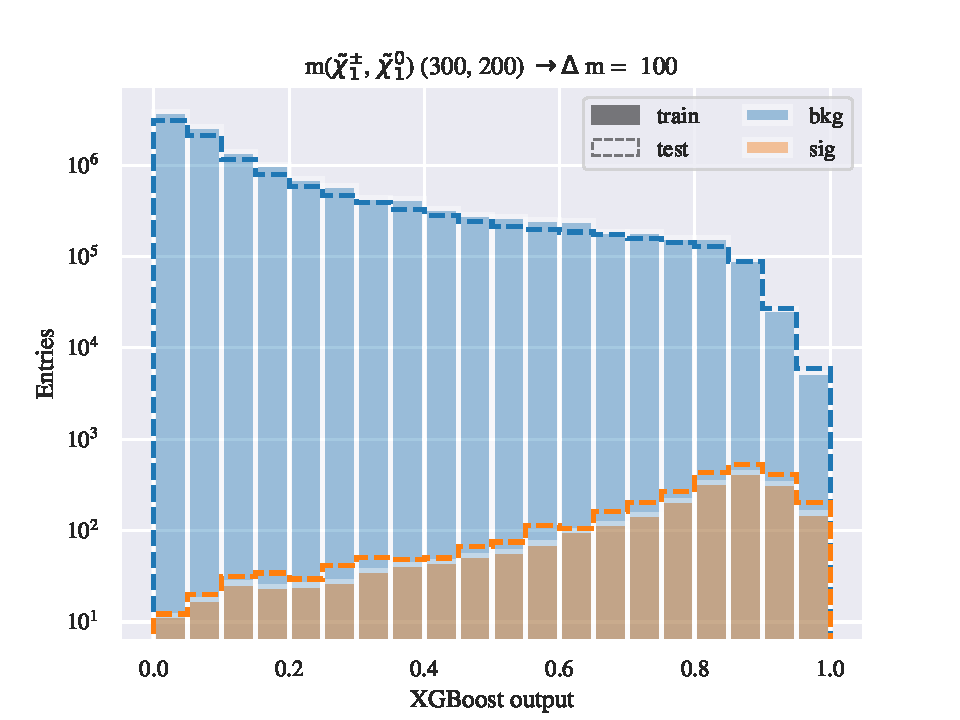
\includegraphics[width = \textwidth]{Figures/SlepSnu/BDT/High_level/Low/scaled_train_test_397115.pdf}
        \caption{Chargino production via $\Tilde{l}/\Tilde{\nu}$.}
        \label{fig:}
    \end{subfigure}
    \begin{subfigure}[t!]{0.49\textwidth}
        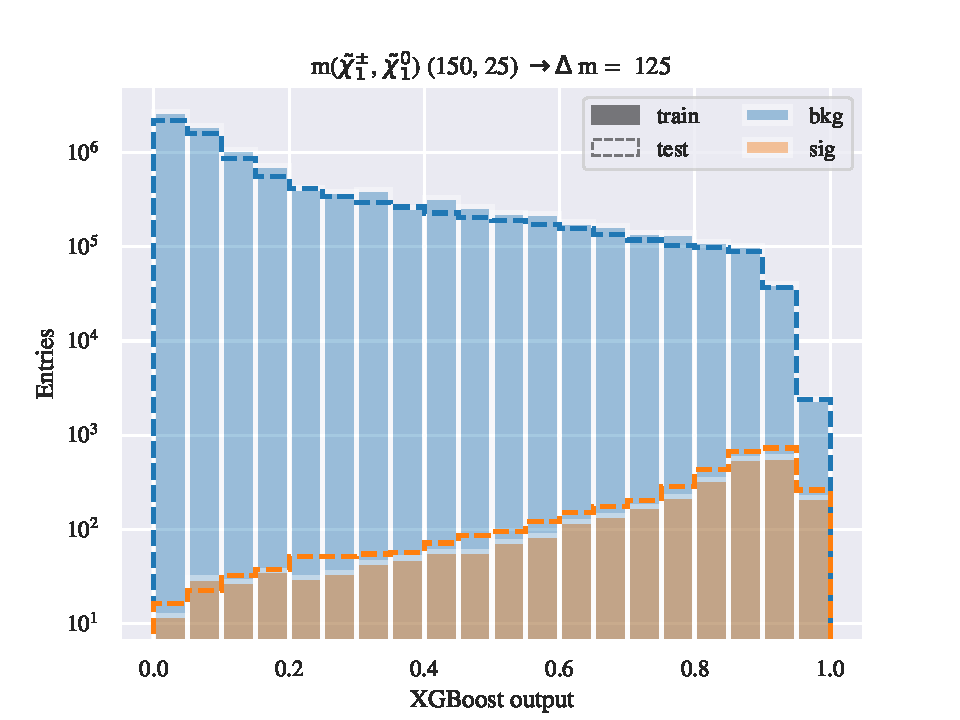
\includegraphics[width = \textwidth]{Figures/WW/BDT/High_level/Low/scaled_train_test_395268.pdf}
        \caption{Chargino production via $W^\pm$.}
        \label{fig:}
    \end{subfigure}
    \begin{subfigure}[t!]{0.49\textwidth}
        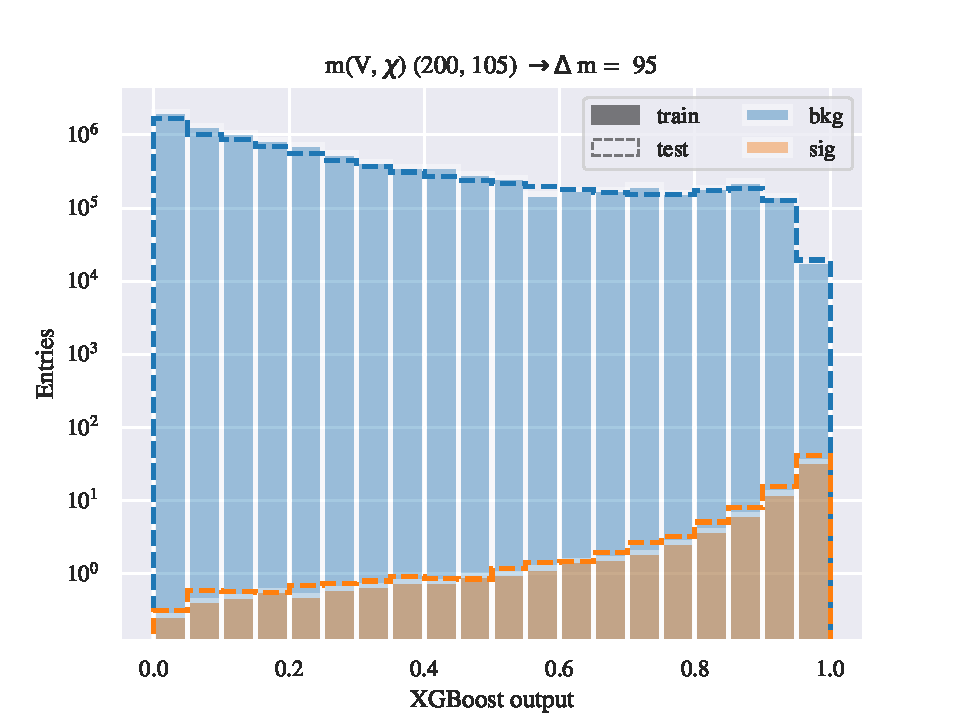
\includegraphics[width = \textwidth]{Figures/Mono_Z/ML/BDT/High_level/Low/scaled_train_test_310604.pdf}
        \caption{Mono-Z.}
        \label{fig:}
    \end{subfigure}
    \caption{Test vs train for low mass splittings done with the BDT using high level features during training. Here the test set is scaled up to match the number of training events.}
    \label{fig:Non}
\end{figure}


\section{Intermediate mass splittings}
\subsection{Low level features}
\begin{figure}[H]
    \centering
    \begin{subfigure}[t!]{0.49\textwidth}
        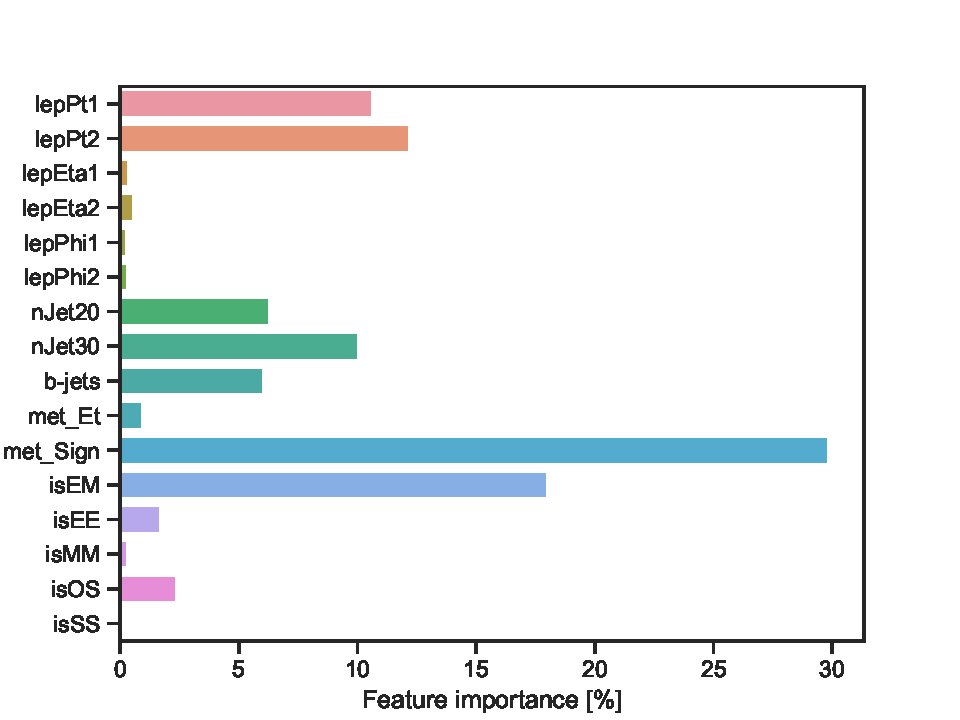
\includegraphics[width = \textwidth]{Figures/SlepSlep/ML/BDT/Low_level/Inter/featureImportance.pdf}
        \caption{Direct slepton production.}
        \label{fig:featSlepslepLow}
    \end{subfigure}
    \begin{subfigure}[t!]{0.49\textwidth}
        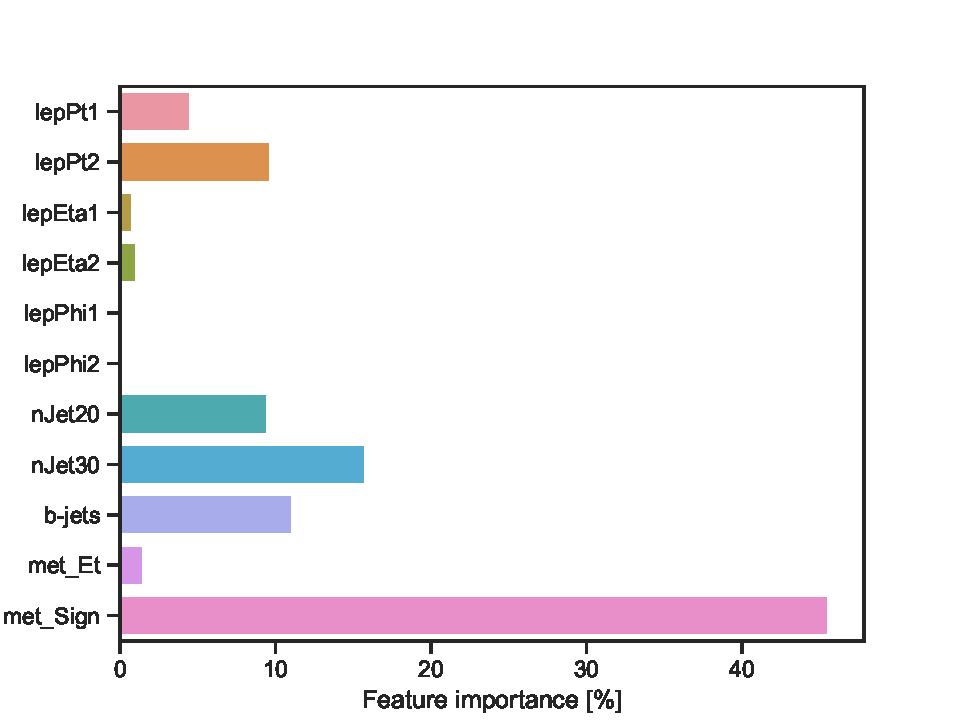
\includegraphics[width = \textwidth]{Figures/SlepSnu/BDT/Low_level/Inter/featureImportance.pdf}
        \caption{Chargino production via $\Tilde{l}/\Tilde{\nu}$.}
        \label{fig:}
    \end{subfigure}
    \begin{subfigure}[t!]{0.49\textwidth}
        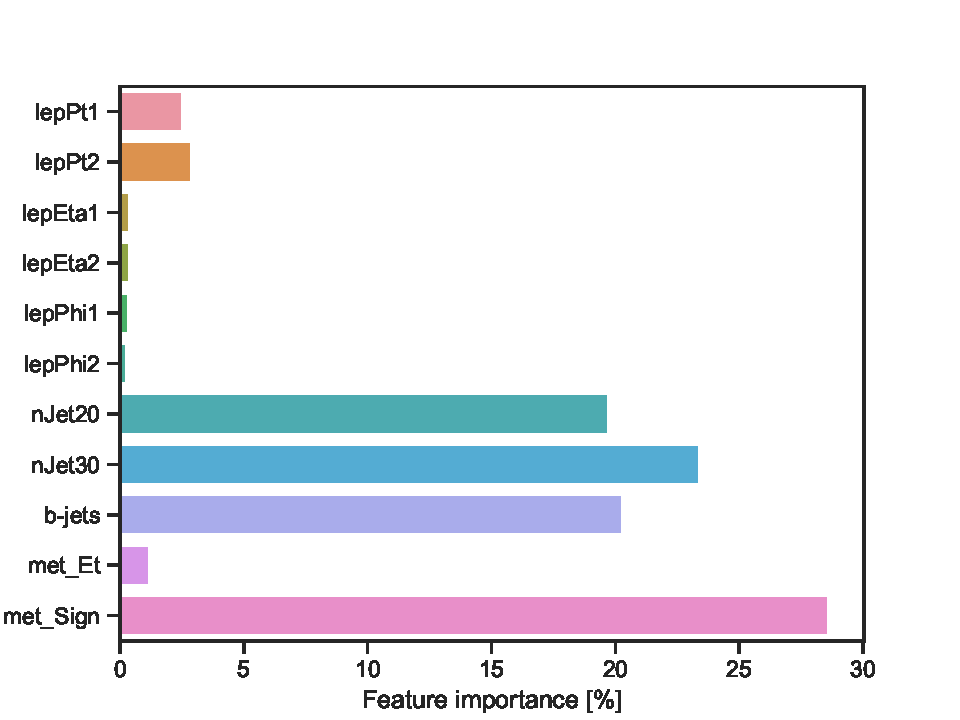
\includegraphics[width = \textwidth]{Figures/WW/BDT/Low_level/Inter/featureImportance.pdf}
        \caption{Chargino production via $W^\pm$.}
        \label{fig:}
    \end{subfigure}
    \begin{subfigure}[t!]{0.49\textwidth}
        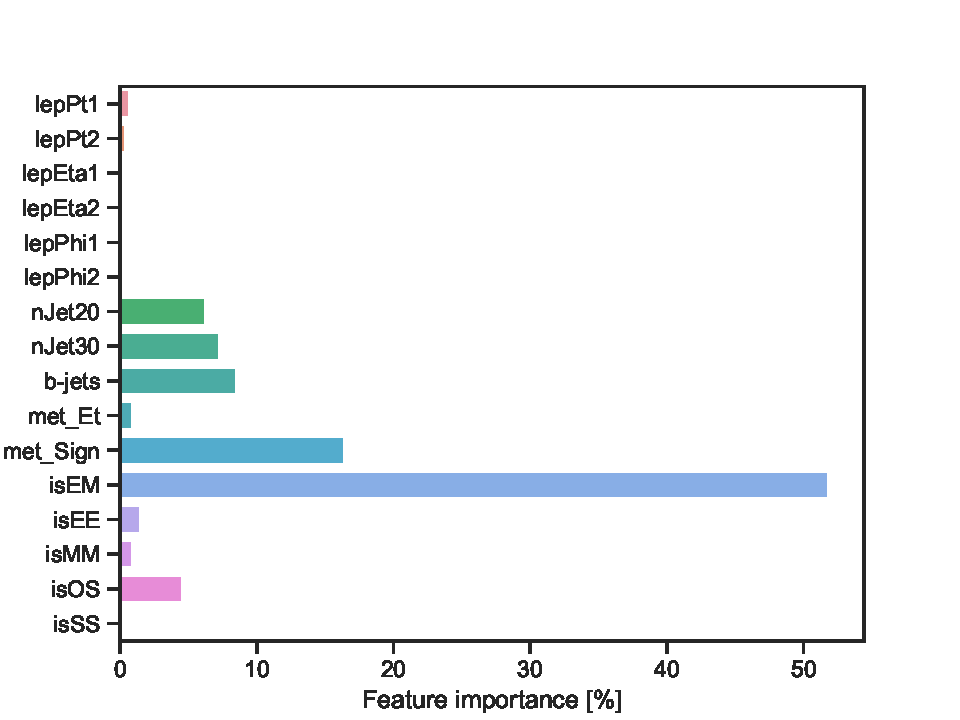
\includegraphics[width = \textwidth]{Figures/Mono_Z/ML/BDT/Low_level/Inter/featureImportance.pdf}
        \caption{Mono-Z.}
        \label{fig:}
    \end{subfigure}
    \caption{Feature importance for low mass splittings for all four processes using low level features during training.}
    \label{fig:Non}
\end{figure}

\begin{figure}[H]
    \centering
    \begin{subfigure}[t!]{0.49\textwidth}
        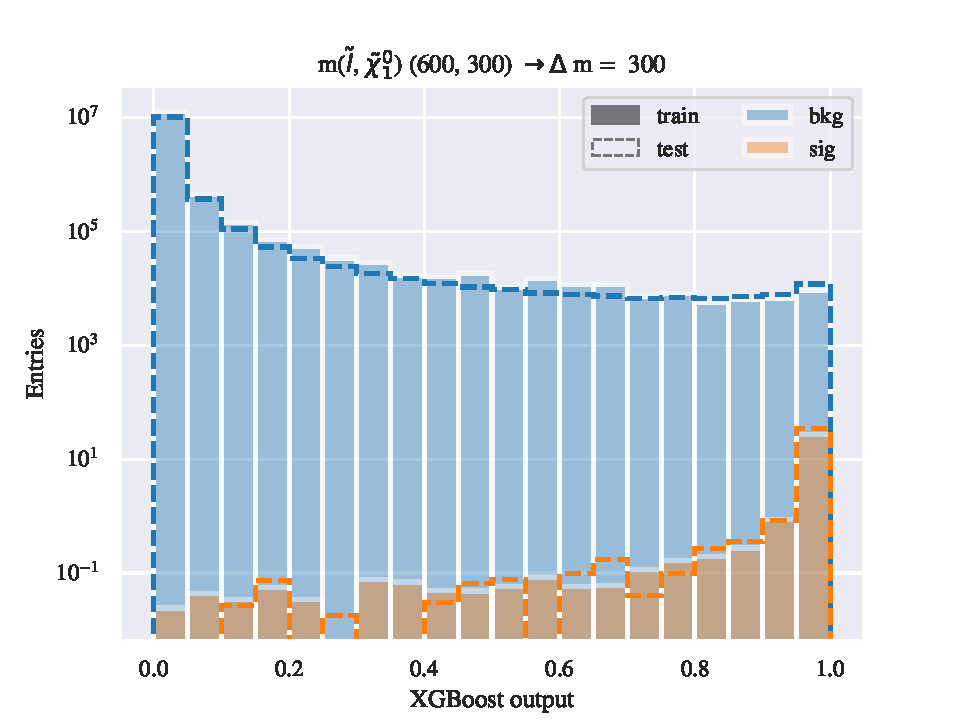
\includegraphics[width = \textwidth]{Figures/SlepSlep/ML/BDT/Low_level/Inter/scaled_train_test_396014.pdf}
        \caption{Direct slepton production.}
        \label{fig:}
    \end{subfigure}
    \begin{subfigure}[t!]{0.49\textwidth}
        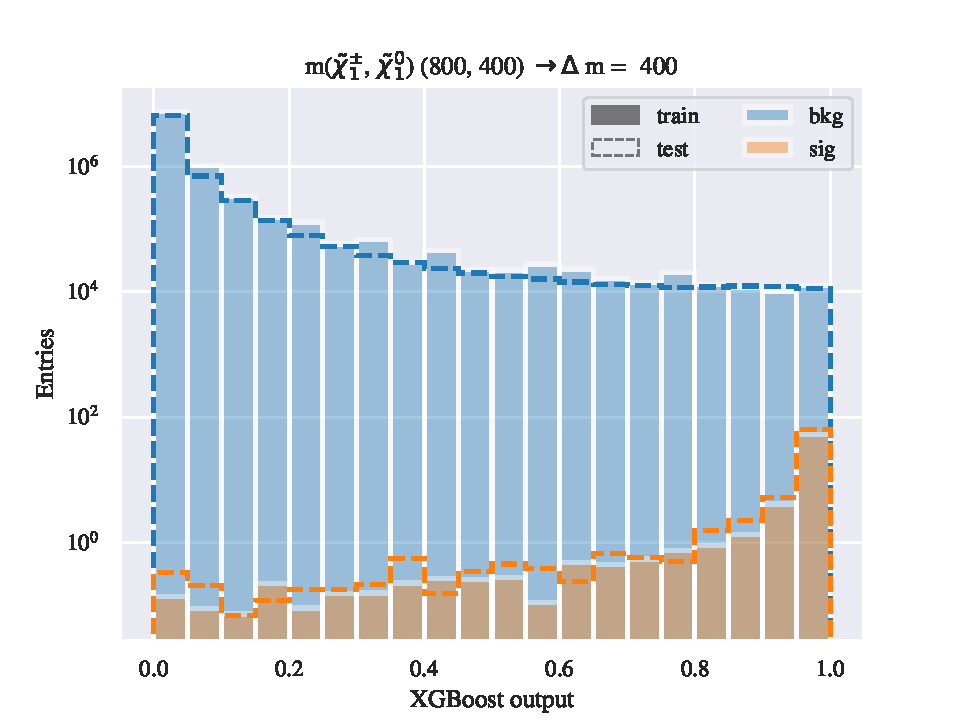
\includegraphics[width = \textwidth]{Figures/SlepSnu/BDT/Low_level/Inter/scaled_train_test_397150.pdf}
        \caption{Chargino production via $\Tilde{l}/\Tilde{\nu}$.}
        \label{fig:}
    \end{subfigure}
    \begin{subfigure}[t!]{0.49\textwidth}
        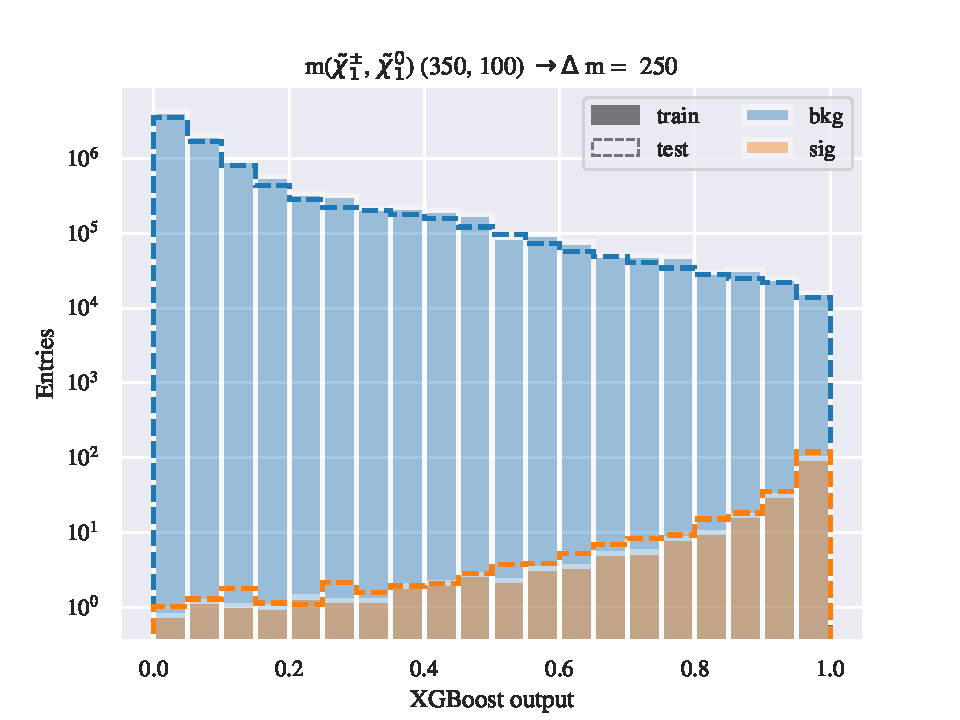
\includegraphics[width = \textwidth]{Figures/WW/BDT/Low_level/Inter/scaled_train_test_395320.pdf}
        \caption{Chargino production via $W^\pm$.}
        \label{fig:}
    \end{subfigure}
    \begin{subfigure}[t!]{0.49\textwidth}
        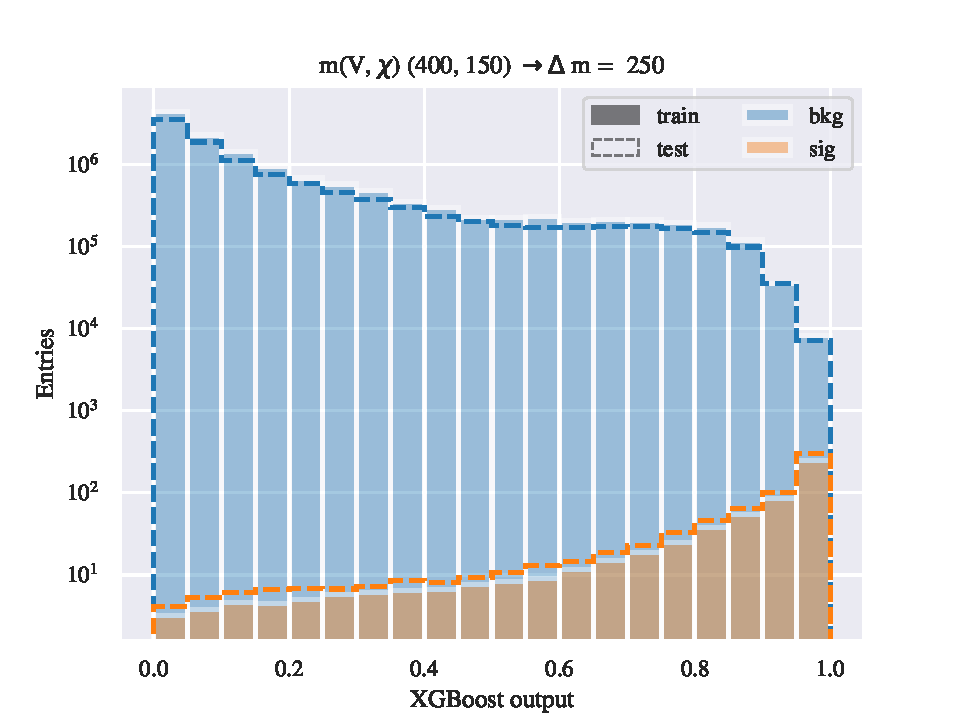
\includegraphics[width = \textwidth]{Figures/Mono_Z/ML/BDT/Low_level/Inter/scaled_train_test_310613.pdf}
        \caption{Mono-Z.}
        \label{fig:}
    \end{subfigure}
    \caption{Test vs train for low mass splittings done with the BDT using low level features during training. Here the test set is scaled up to match the number of training events.}
    \label{fig:Non}
\end{figure}



\subsection{High level features}

\begin{figure}[H]
    \centering
    \begin{subfigure}[t!]{0.49\textwidth}
        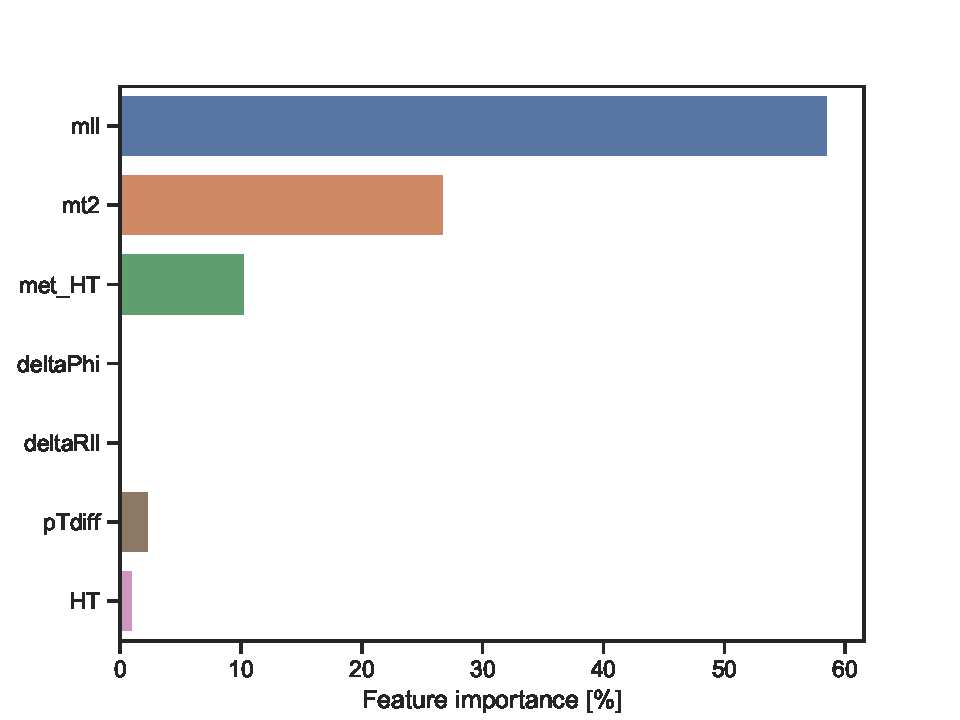
\includegraphics[width = \textwidth]{Figures/SlepSlep/ML/BDT/High_level/Inter/featureImportance.pdf}
        \caption{Direct slepton production.}
        \label{fig:}
    \end{subfigure}
    \begin{subfigure}[t!]{0.49\textwidth}
        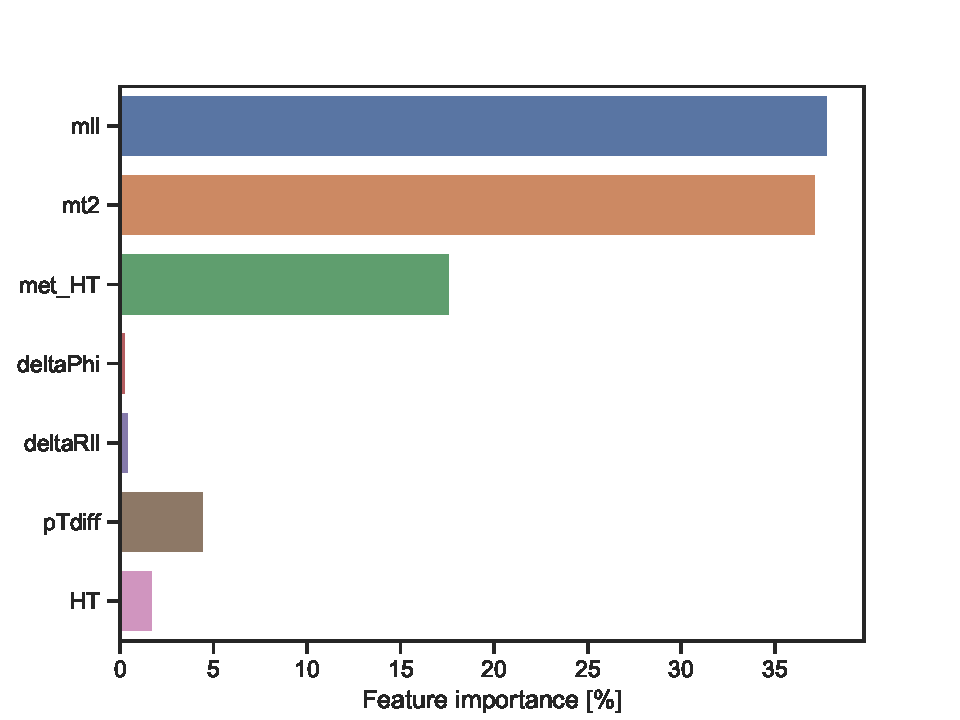
\includegraphics[width = \textwidth]{Figures/SlepSnu/BDT/High_level/Inter/featureImportance.pdf}
        \caption{Chargino production via $\Tilde{l}/\Tilde{\nu}$.}
        \label{fig:}
    \end{subfigure}
    \begin{subfigure}[t!]{0.49\textwidth}
        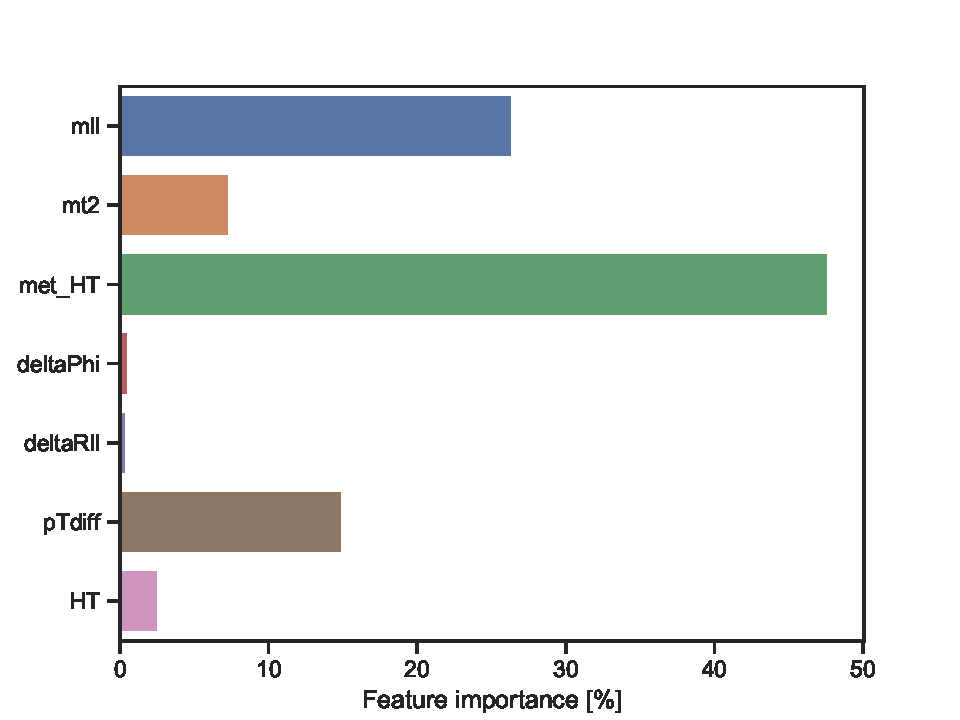
\includegraphics[width = \textwidth]{Figures/WW/BDT/High_level/Inter/featureImportance.pdf}
        \caption{Chargino production via $W^\pm$.}
        \label{fig:}
    \end{subfigure}
    \begin{subfigure}[t!]{0.49\textwidth}
        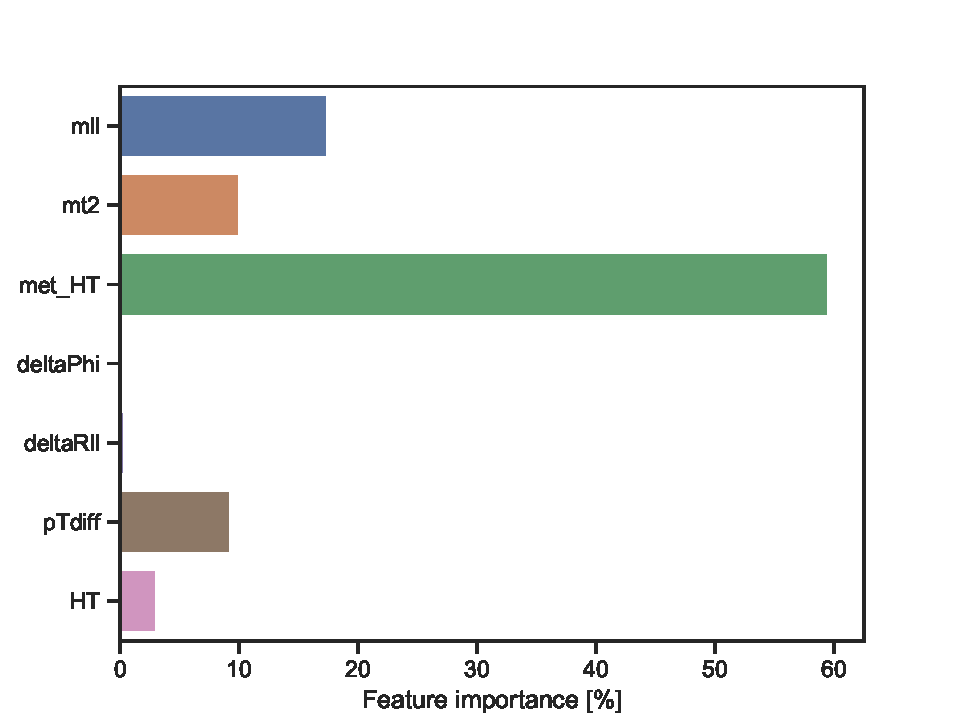
\includegraphics[width = \textwidth]{Figures/Mono_Z/ML/BDT/High_level/Inter/featureImportance.pdf}
        \caption{Mono-Z.}
        \label{fig:}
    \end{subfigure}
    \caption{Feature importance for low mass splittings for all four processes using high level features during training.}
    \label{fig:Non}
\end{figure}

\begin{figure}[H]
    \centering
    \begin{subfigure}[t!]{0.49\textwidth}
        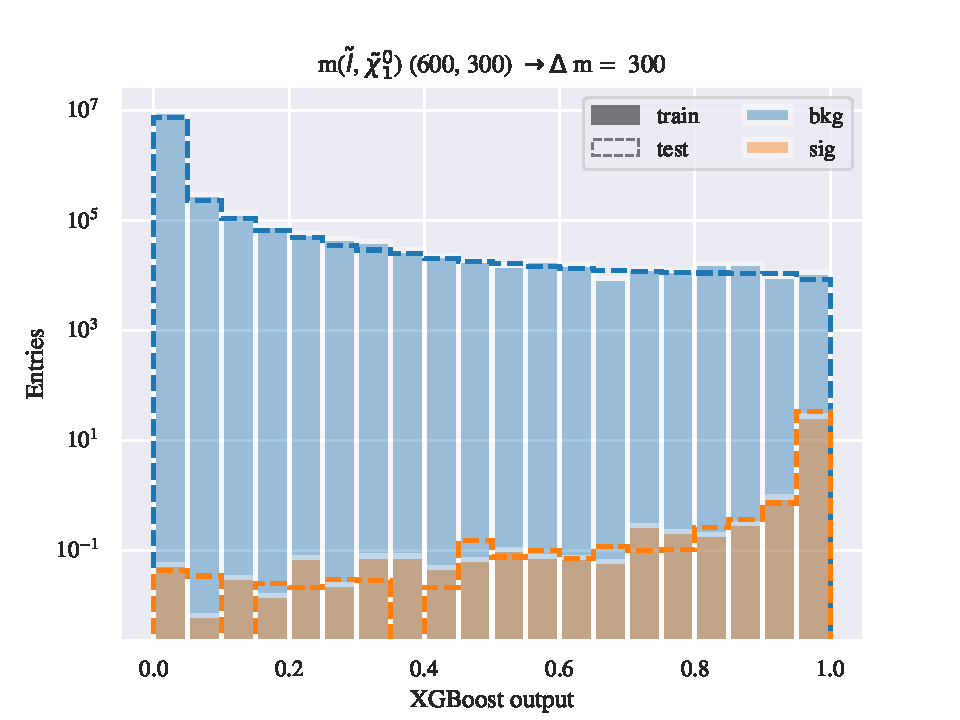
\includegraphics[width = \textwidth]{Figures/SlepSlep/ML/BDT/High_level/Inter/scaled_train_test_396014.pdf}
        \caption{Direct slepton production.}
        \label{fig:}
    \end{subfigure}
    \begin{subfigure}[t!]{0.49\textwidth}
        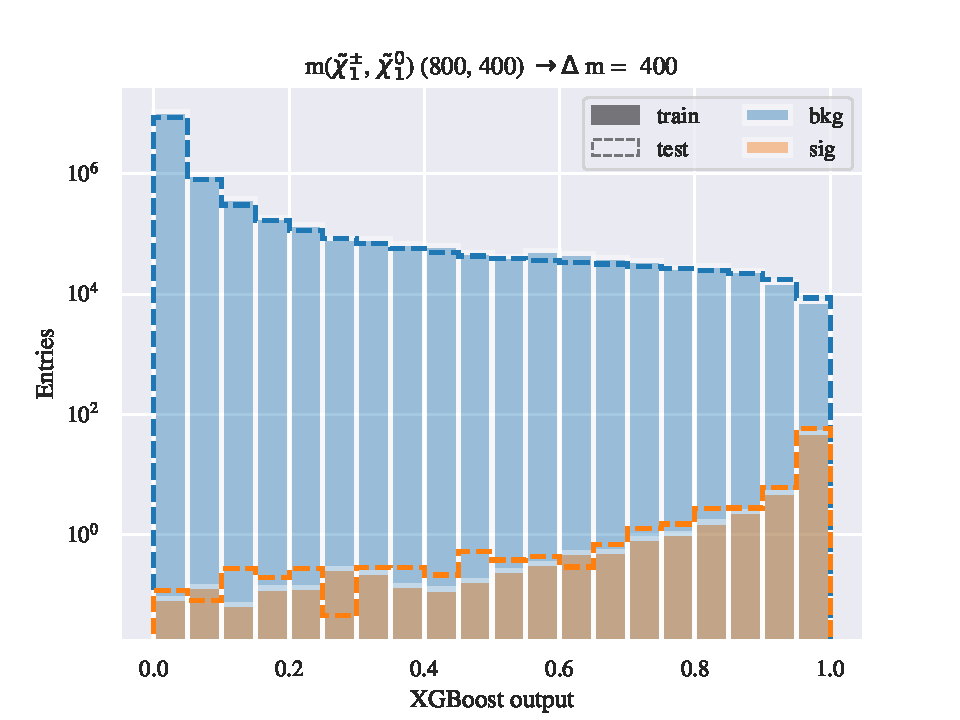
\includegraphics[width = \textwidth]{Figures/SlepSnu/BDT/High_level/Inter/scaled_train_test_397150.pdf}
        \caption{Chargino production via $\Tilde{l}/\Tilde{\nu}$.}
        \label{fig:}
    \end{subfigure}
    \begin{subfigure}[t!]{0.49\textwidth}
        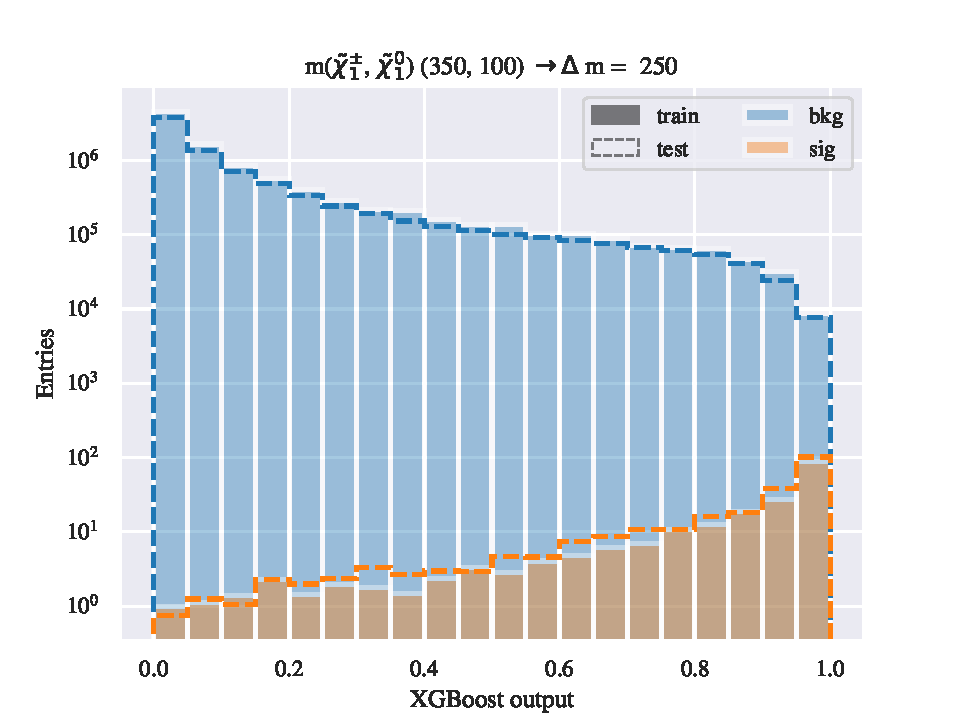
\includegraphics[width = \textwidth]{Figures/WW/BDT/High_level/Inter/scaled_train_test_395320.pdf}
        \caption{Chargino production via $W^\pm$.}
        \label{fig:}
    \end{subfigure}
    \begin{subfigure}[t!]{0.49\textwidth}
        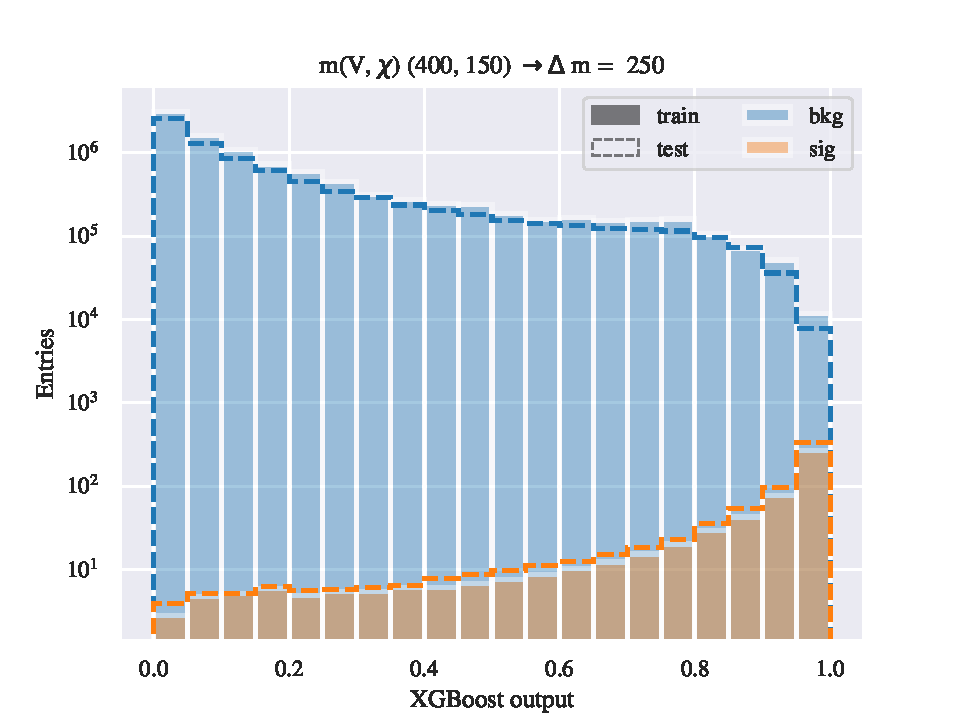
\includegraphics[width = \textwidth]{Figures/Mono_Z/ML/BDT/High_level/Inter/scaled_train_test_310613.pdf}
        \caption{Mono-Z.}
        \label{fig:}
    \end{subfigure}
    \caption{Test vs train for low mass splittings done with the BDT using high level features during training. Here the test set is scaled up to match the number of training events.}
    \label{fig:Non}
\end{figure}




\section{High mass splittings}
\subsection{Low level features}
\begin{figure}[H]
    \centering
    \begin{subfigure}[t!]{0.49\textwidth}
        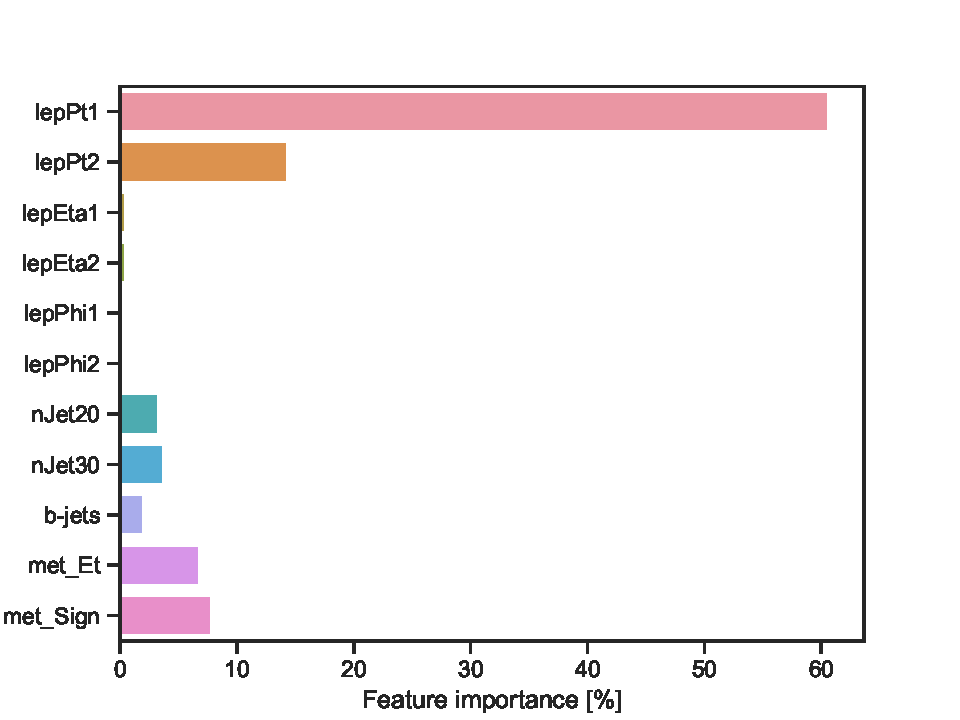
\includegraphics[width = \textwidth]{Figures/SlepSlep/ML/BDT/Low_level/High/featureImportance.pdf}
        \caption{Direct slepton production.}
        \label{fig:}
    \end{subfigure}
    \begin{subfigure}[t!]{0.49\textwidth}
        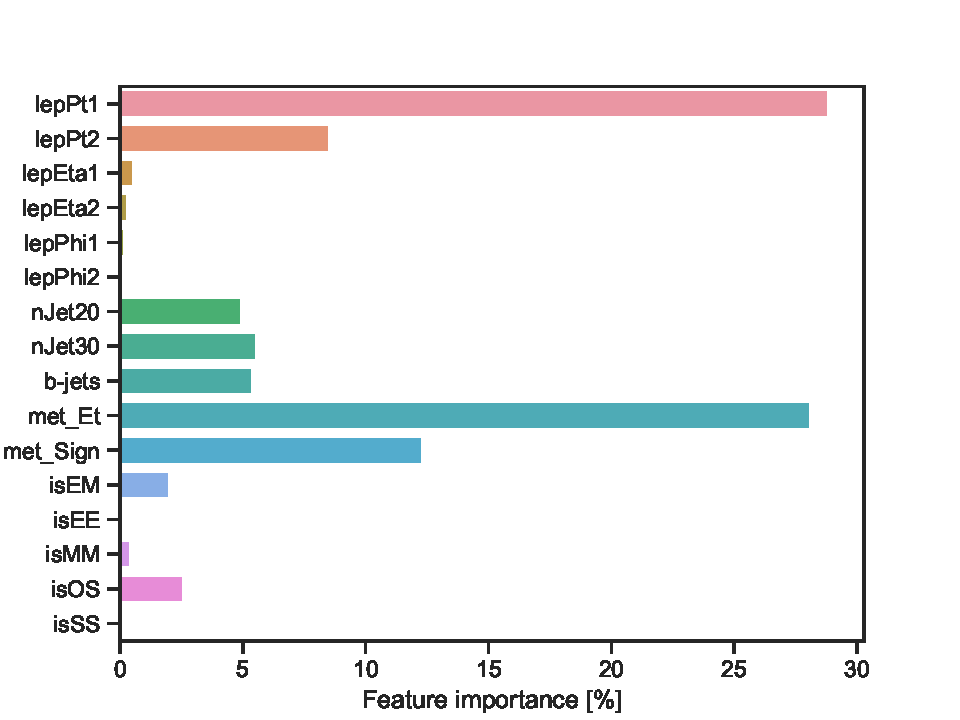
\includegraphics[width = \textwidth]{Figures/SlepSnu/BDT/Low_level/High/featureImportance.pdf}
        \caption{Chargino production via $\Tilde{l}/\Tilde{\nu}$.}
        \label{fig:}
    \end{subfigure}
    \begin{subfigure}[t!]{0.49\textwidth}
        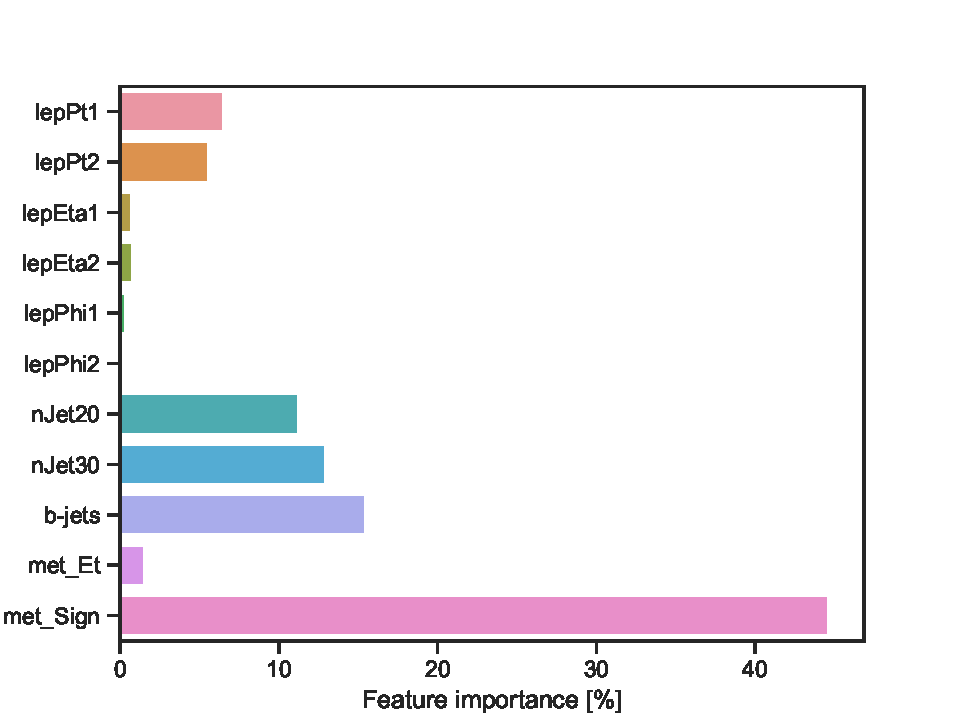
\includegraphics[width = \textwidth]{Figures/WW/BDT/Low_level/High/featureImportance.pdf}
        \caption{Chargino production via $W^\pm$.}
        \label{fig:}
    \end{subfigure}
    \begin{subfigure}[t!]{0.49\textwidth}
        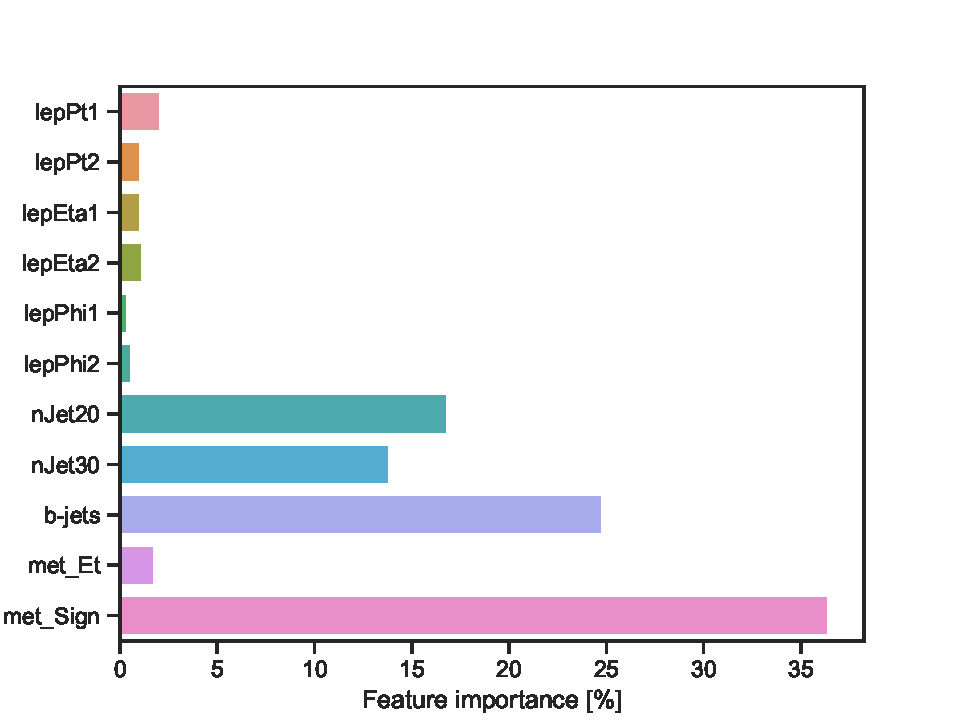
\includegraphics[width = \textwidth]{Figures/Mono_Z/ML/BDT/Low_level/High/featureImportance.pdf}
        \caption{Mono-Z.}
        \label{fig:}
    \end{subfigure}
    \caption{Feature importance for low mass splittings for all four processes using low level features during training.}
    \label{fig:Non}
\end{figure}


\begin{figure}[H]
    \centering
    \begin{subfigure}[t!]{0.49\textwidth}
        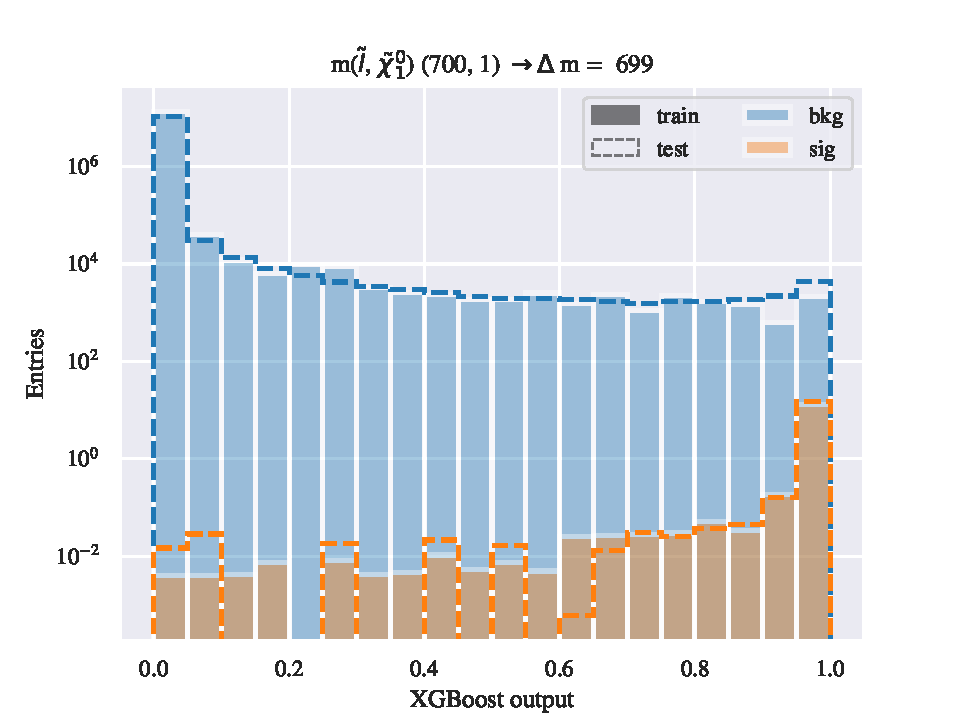
\includegraphics[width = \textwidth]{Figures/SlepSlep/ML/BDT/Low_level/High/scaled_train_test_396033.pdf}
        \caption{Direct slepton production.}
        \label{fig:}
    \end{subfigure}
    \begin{subfigure}[t!]{0.49\textwidth}
        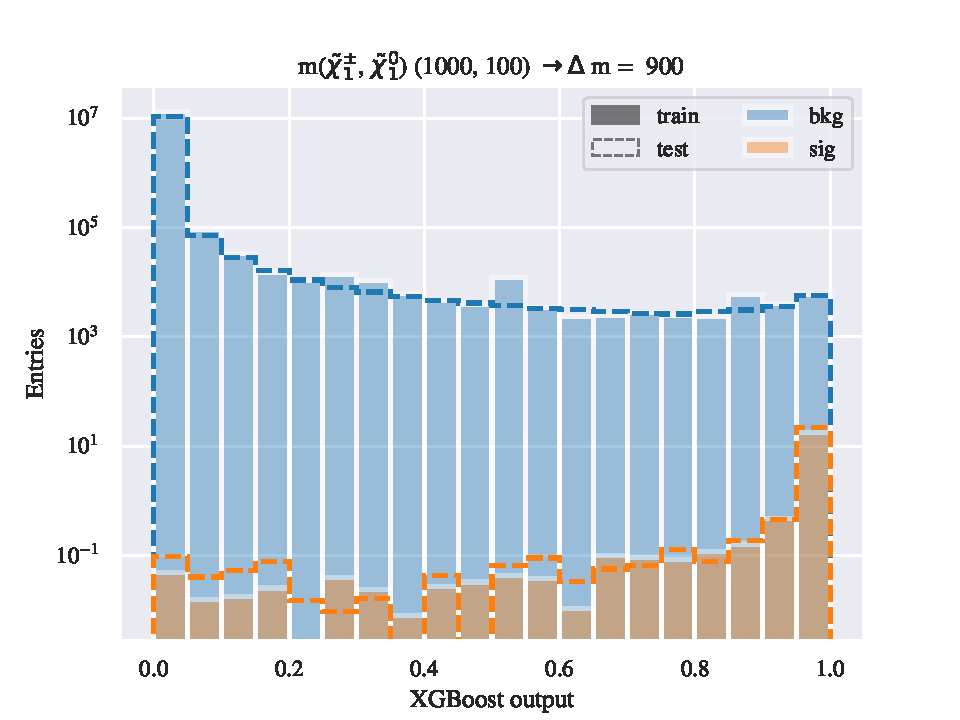
\includegraphics[width = \textwidth]{Figures/SlepSnu/BDT/Low_level/High/scaled_train_test_397169.pdf}
        \caption{Chargino production via $\Tilde{l}/\Tilde{\nu}$.}
        \label{fig:}
    \end{subfigure}
    \begin{subfigure}[t!]{0.49\textwidth}
        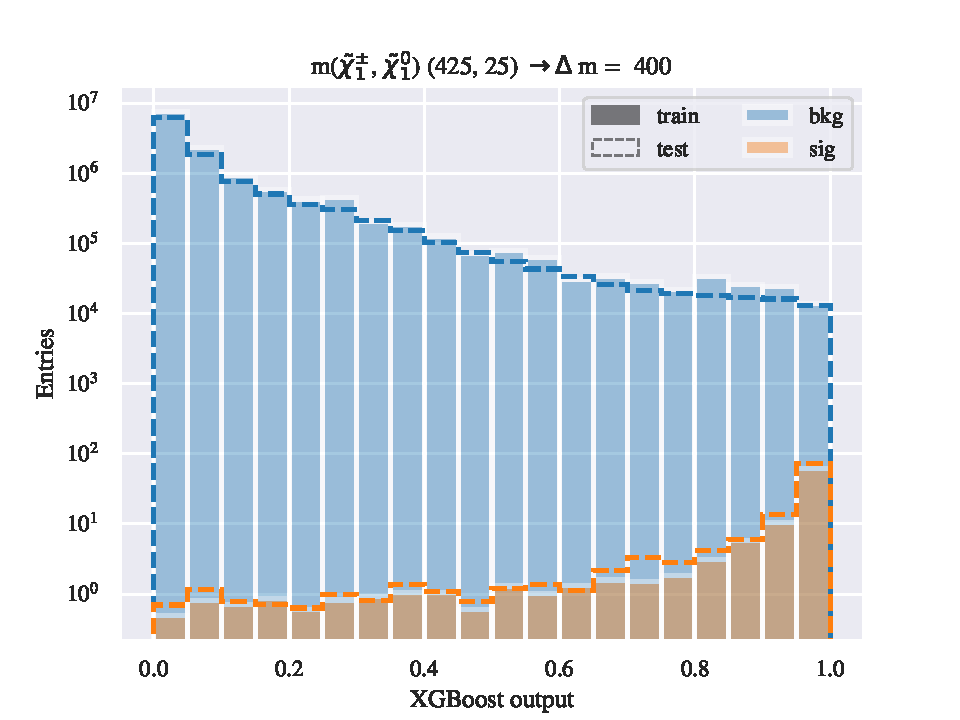
\includegraphics[width = \textwidth]{Figures/WW/BDT/Low_level/High/scaled_train_test_395330.pdf}
        \caption{Chargino production via $W^\pm$.}
        \label{fig:}
    \end{subfigure}
    \begin{subfigure}[t!]{0.49\textwidth}
        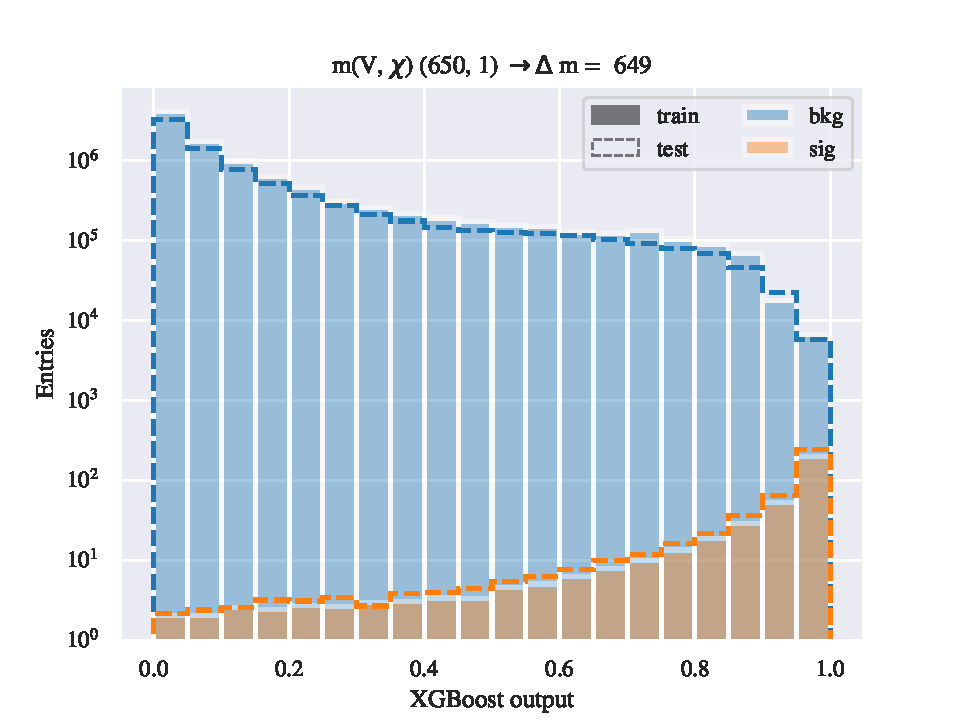
\includegraphics[width = \textwidth]{Figures/Mono_Z/ML/BDT/Low_level/High/scaled_train_test_310617.pdf}
        \caption{Mono-Z.}
        \label{fig:}
    \end{subfigure}
    \caption{Test vs train for low mass splittings done with the BDT using low level features during training. Here the test set is scaled up to match the number of training events.}
    \label{fig:Non}
\end{figure}


\subsection{High level features}
\begin{figure}[H]
    \centering
    \begin{subfigure}[t!]{0.49\textwidth}
        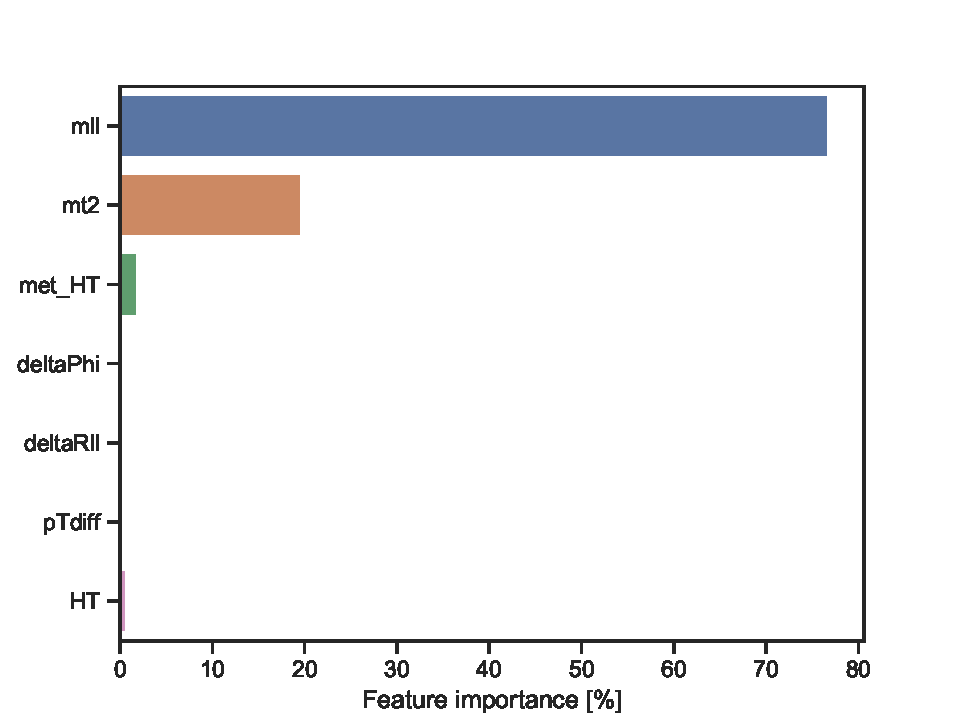
\includegraphics[width = \textwidth]{Figures/SlepSlep/ML/BDT/High_level/High/featureImportance.pdf}
        \caption{Direct slepton production.}
        \label{fig:}
    \end{subfigure}
    \begin{subfigure}[t!]{0.49\textwidth}
        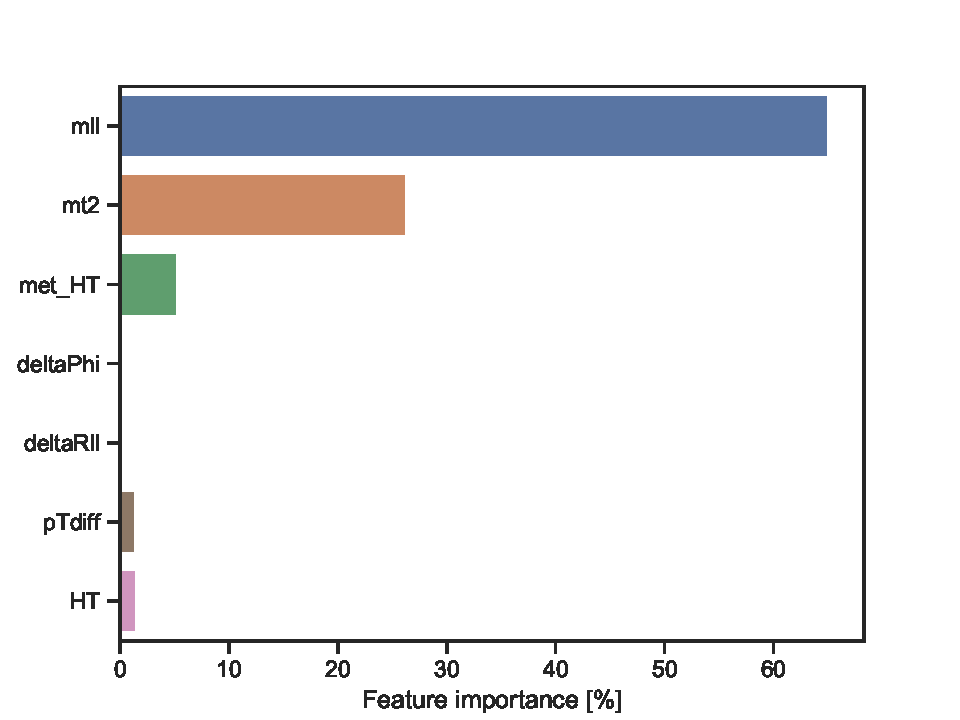
\includegraphics[width = \textwidth]{Figures/SlepSnu/BDT/High_level/High/featureImportance.pdf}
        \caption{Chargino production via $\Tilde{l}/\Tilde{\nu}$.}
        \label{fig:}
    \end{subfigure}
    \begin{subfigure}[t!]{0.49\textwidth}
        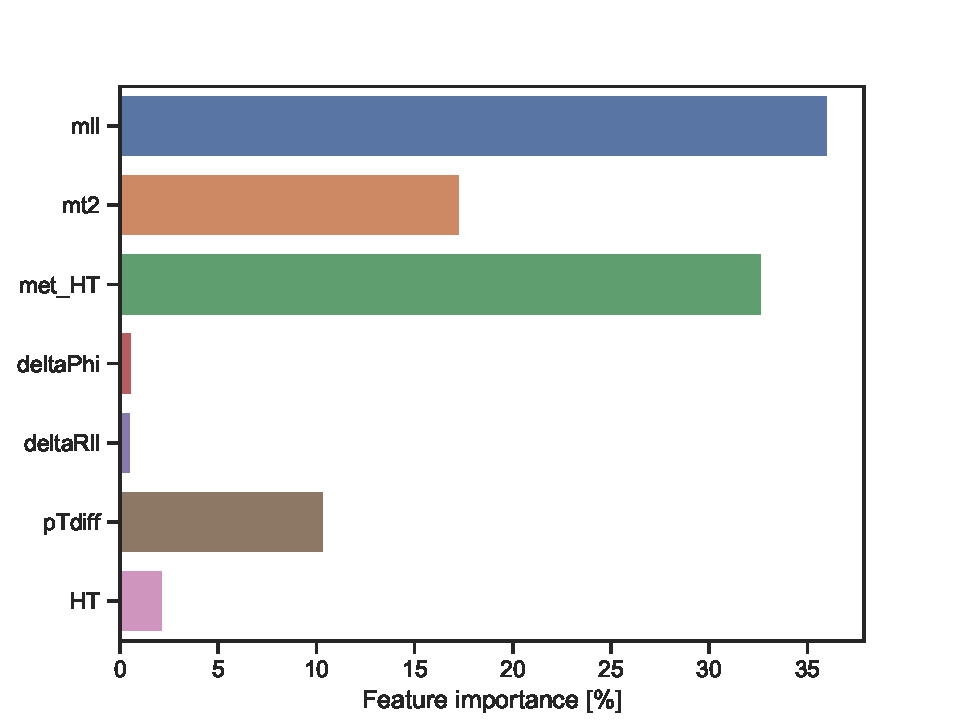
\includegraphics[width = \textwidth]{Figures/WW/BDT/High_level/High/featureImportance.pdf}
        \caption{Chargino production via $W^\pm$.}
        \label{fig:}
    \end{subfigure}
    \begin{subfigure}[t!]{0.49\textwidth}
        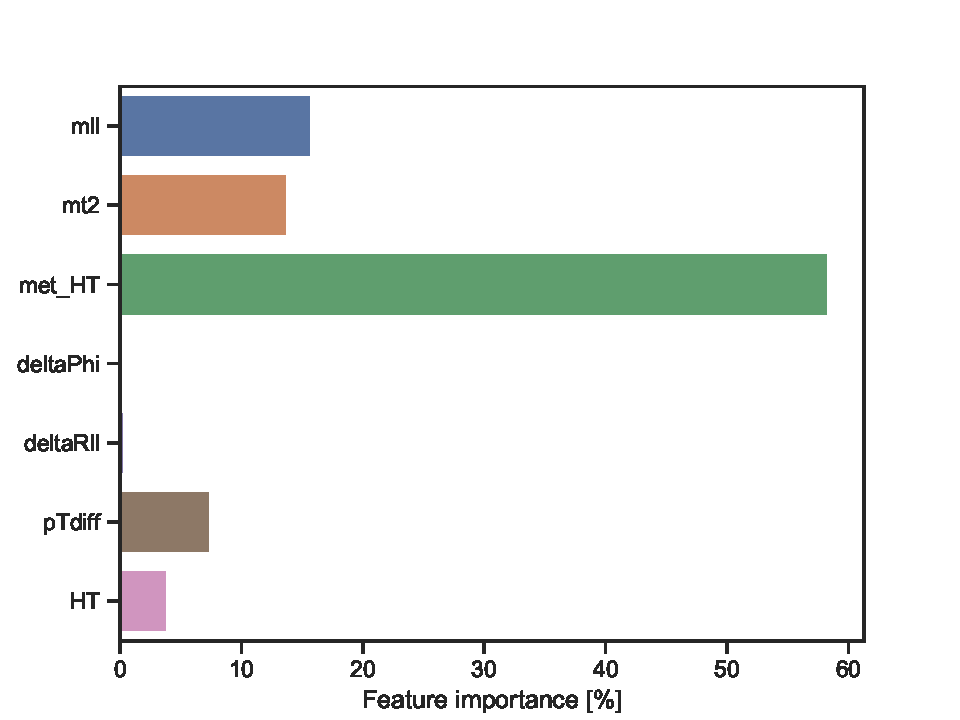
\includegraphics[width = \textwidth]{Figures/Mono_Z/ML/BDT/High_level/High/featureImportance.pdf}
        \caption{Mono-Z.}
        \label{fig:}
    \end{subfigure}
    \caption{Feature importance for low mass splittings for all four processes using high level features during training.}
    \label{fig:Non}
\end{figure}



\begin{figure}[H]
    \centering
    \begin{subfigure}[t!]{0.49\textwidth}
        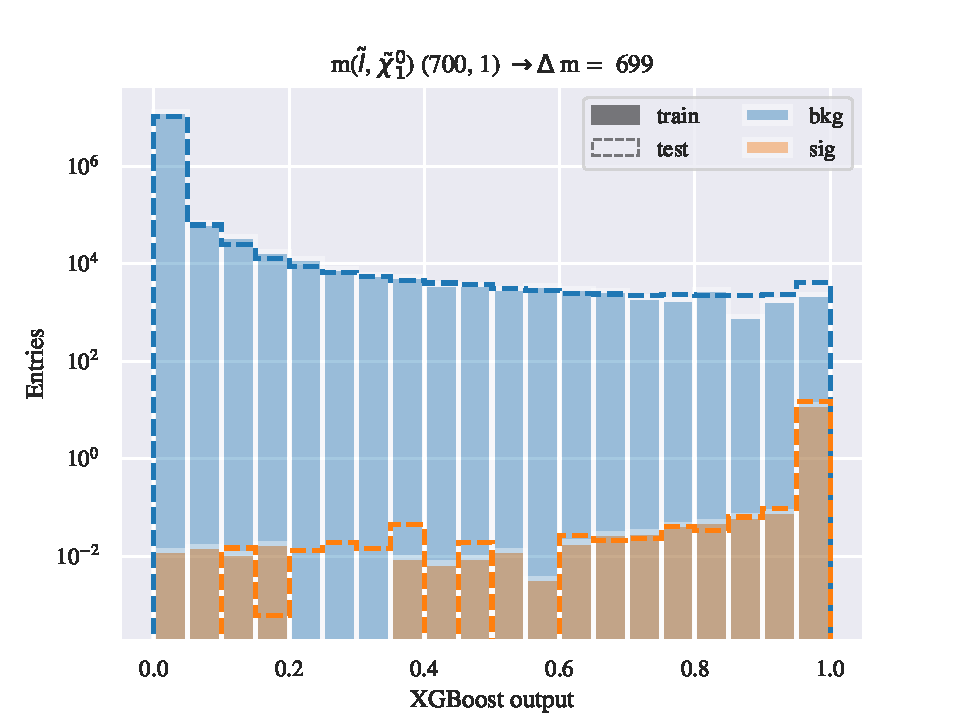
\includegraphics[width = \textwidth]{Figures/SlepSlep/ML/BDT/High_level/High/scaled_train_test_396033.pdf}
        \caption{Direct slepton production.}
        \label{fig:}
    \end{subfigure}
    \begin{subfigure}[t!]{0.49\textwidth}
        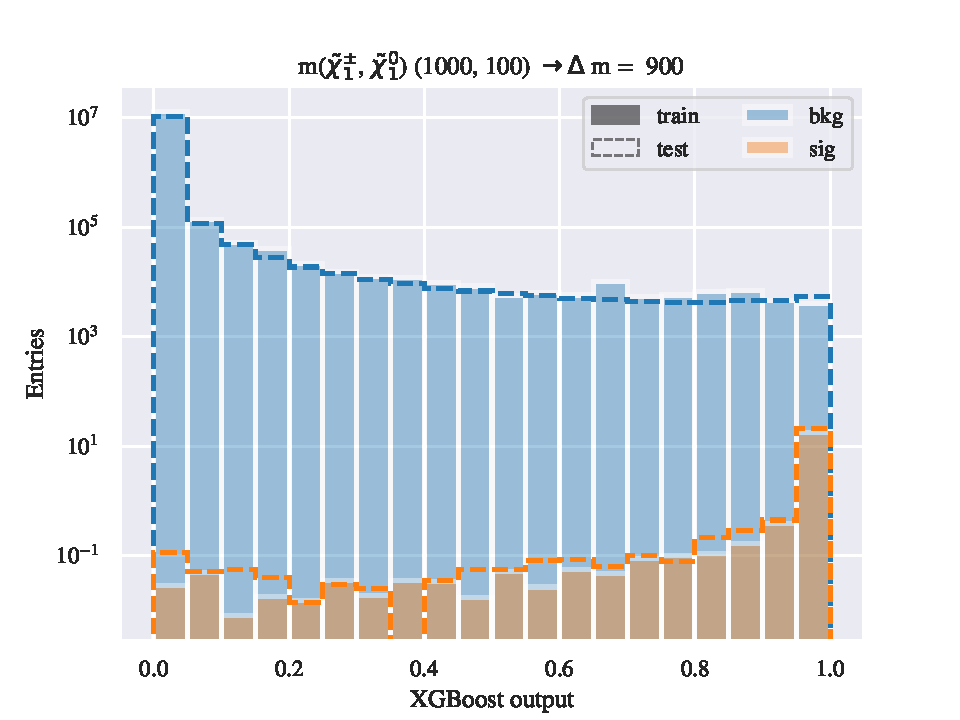
\includegraphics[width = \textwidth]{Figures/SlepSnu/BDT/High_level/High/scaled_train_test_397169.pdf}
        \caption{Chargino production via $\Tilde{l}/\Tilde{\nu}$.}
        \label{fig:}
    \end{subfigure}
    \begin{subfigure}[t!]{0.49\textwidth}
        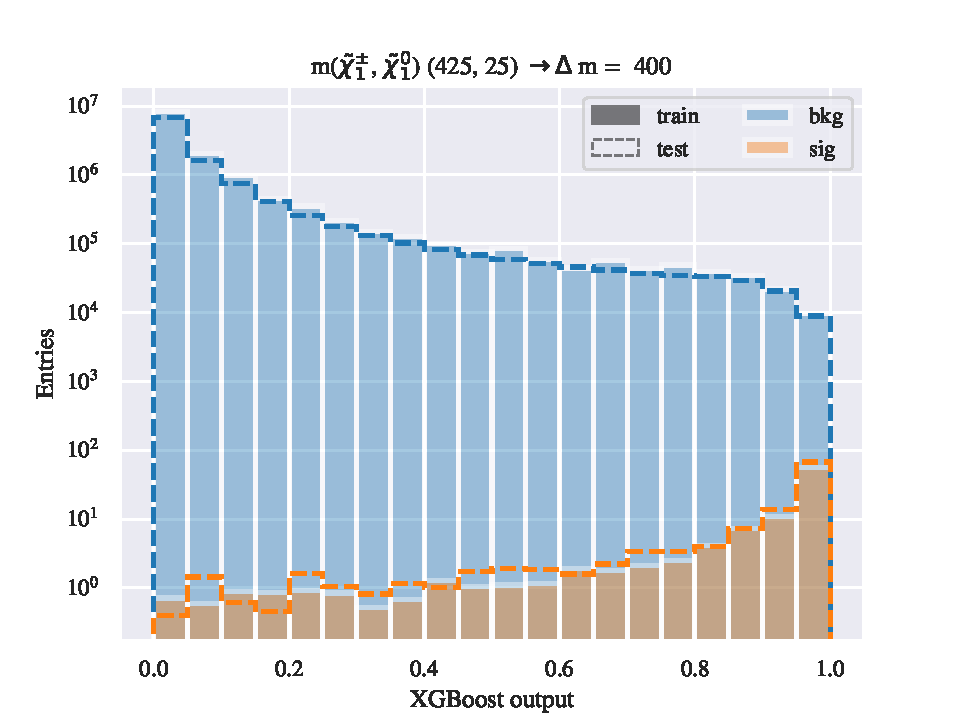
\includegraphics[width = \textwidth]{Figures/WW/BDT/High_level/High/scaled_train_test_395330.pdf}
        \caption{Chargino production via $W^\pm$.}
        \label{fig:}
    \end{subfigure}
    \begin{subfigure}[t!]{0.49\textwidth}
        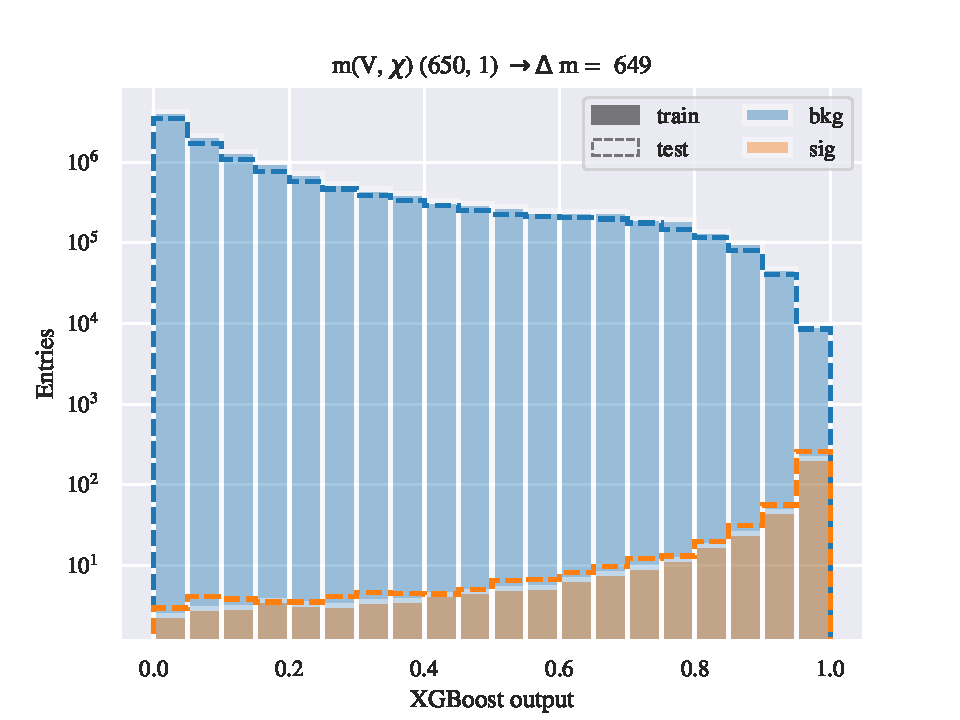
\includegraphics[width = \textwidth]{Figures/Mono_Z/ML/BDT/High_level/High/scaled_train_test_310617.pdf}
        \caption{Mono-Z.}
        \label{fig:}
    \end{subfigure}
    \caption{Test vs train for low mass splittings done with the BDT using high level features during training. Here the test set is scaled up to match the number of training events.}
    \label{fig:Non}
\end{figure}




\section{Stacked background with data}
\subsection{Low level features}

\begin{figure}[H]
    \centering
    \begin{subfigure}[t!]{0.49\textwidth}
        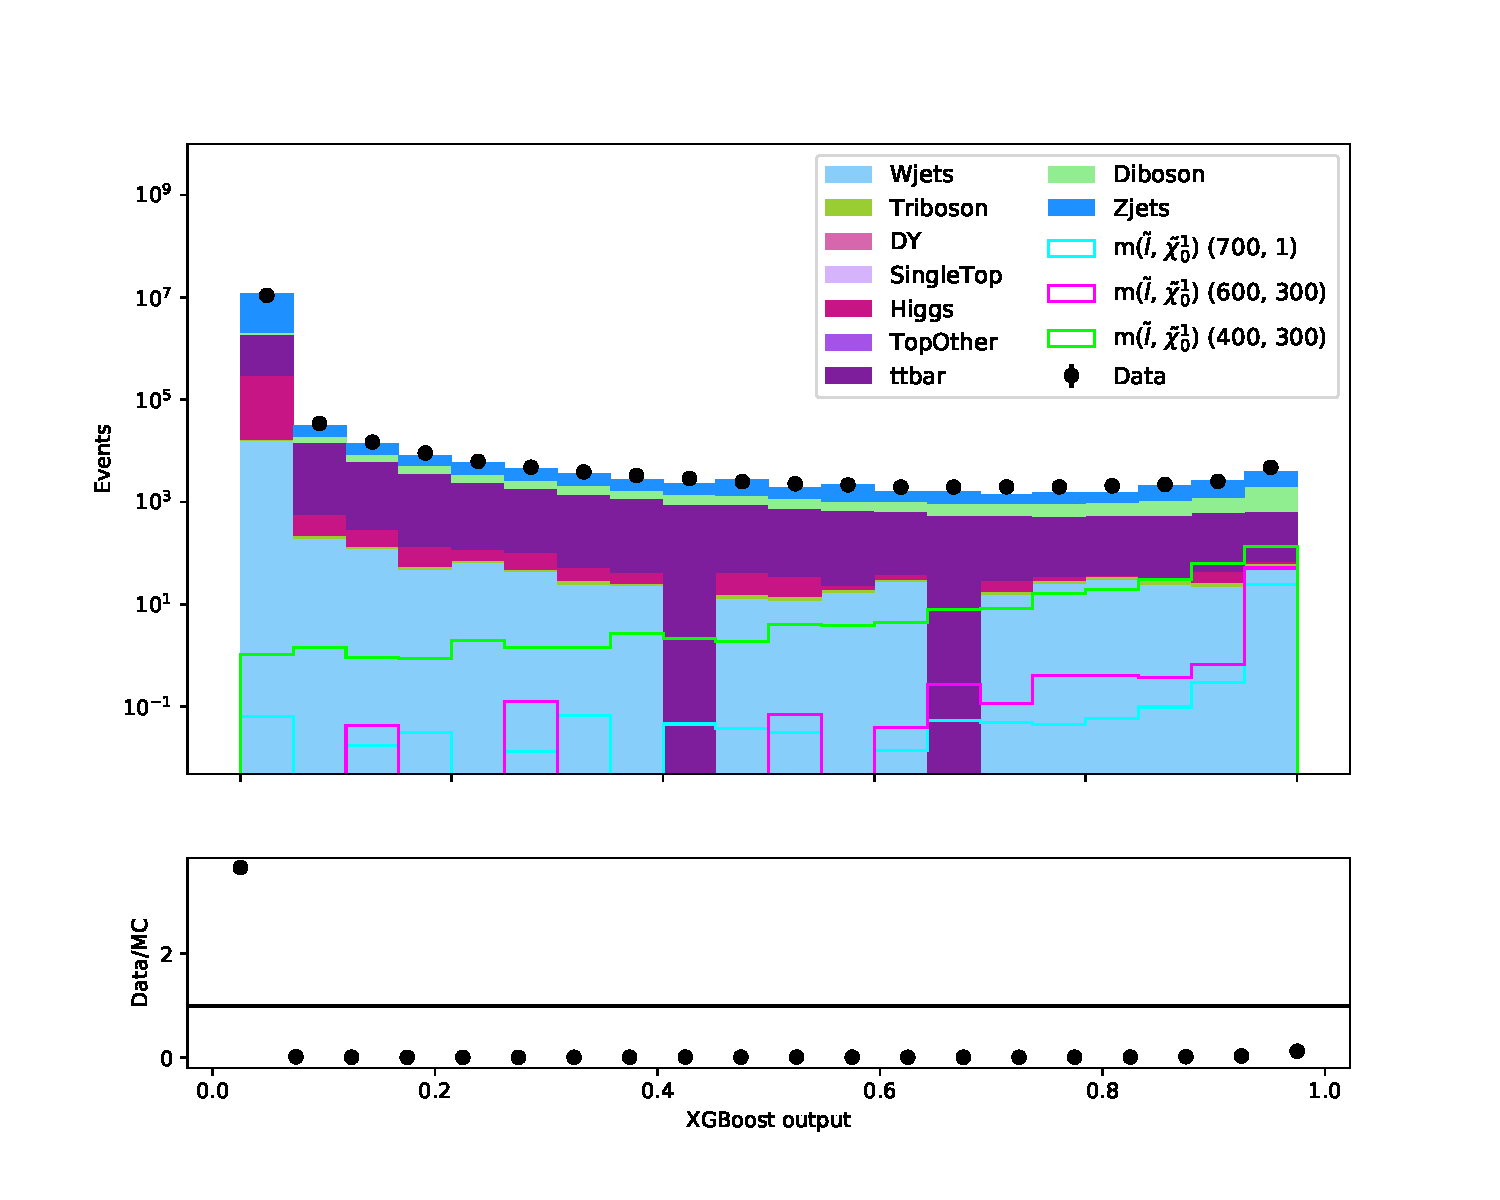
\includegraphics[width = \textwidth]{Figures/Stacked/stackedplot_BDT_Low_level_slepslep.pdf}
        \caption{Direct slepton production.}
        \label{fig:}
    \end{subfigure}
    \begin{subfigure}[t!]{0.49\textwidth}
        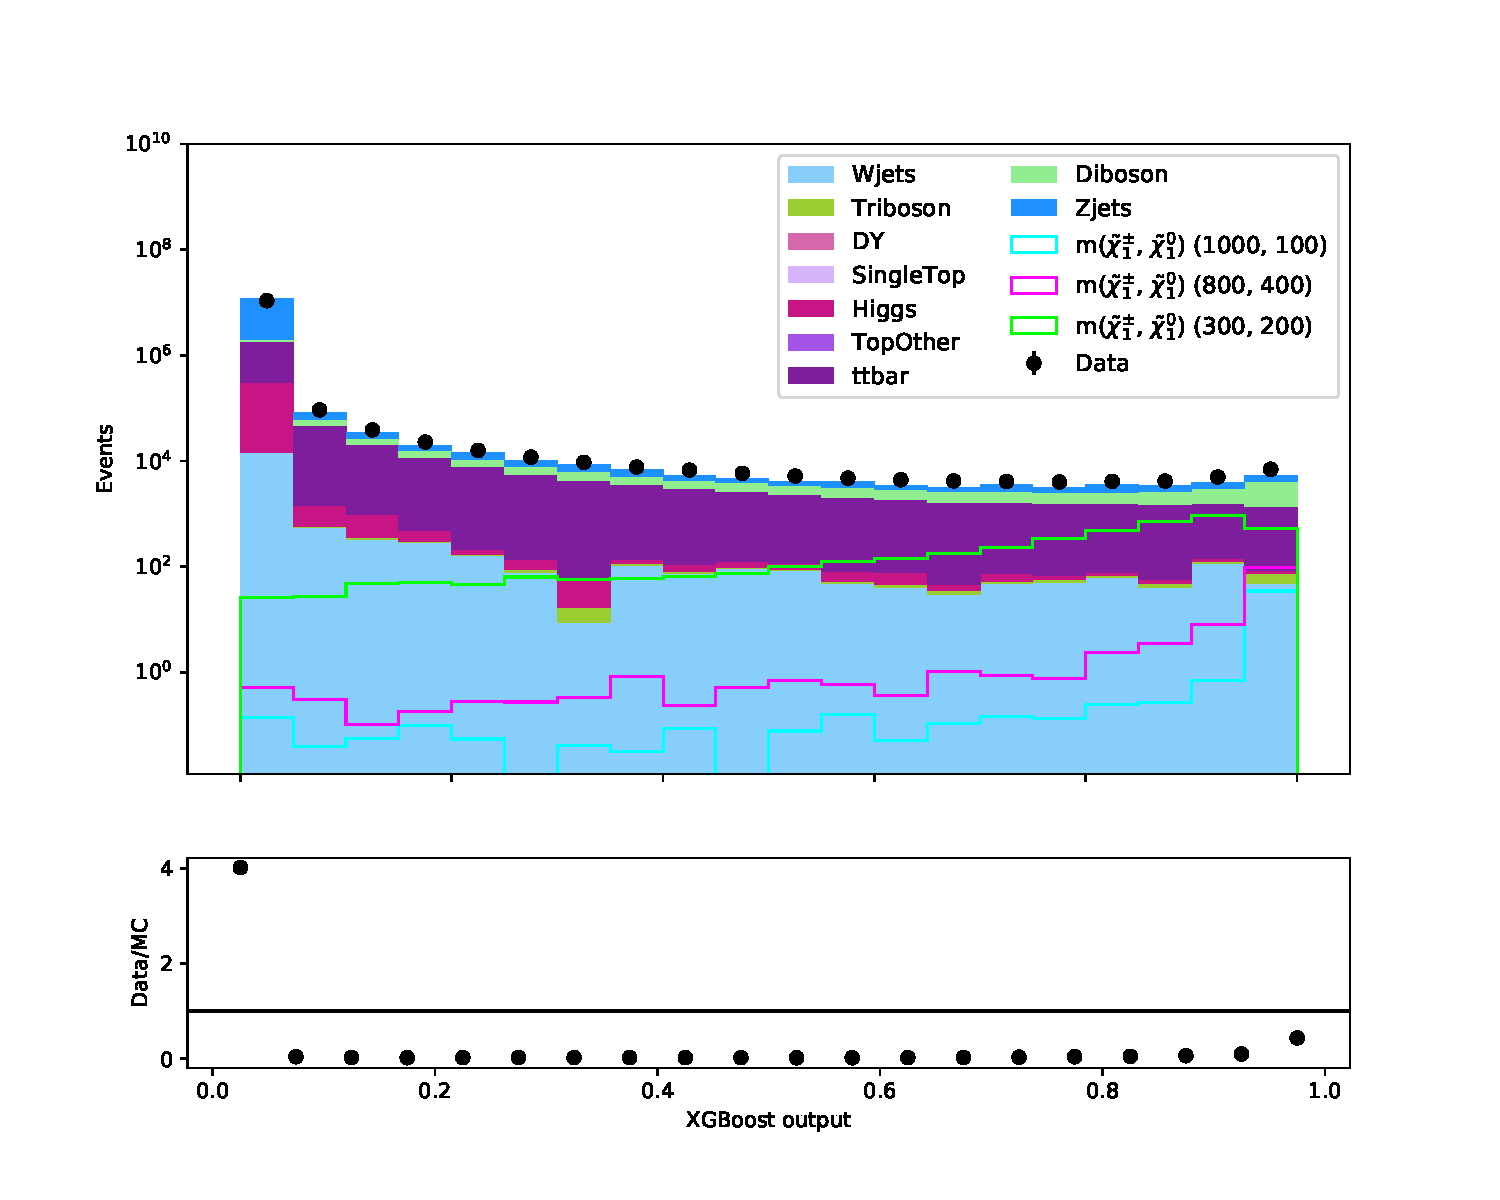
\includegraphics[width = \textwidth]{Figures/Stacked/stackedplot_BDT_Low_level_slepsnu.pdf}
        \caption{Chargino production via $\Tilde{l}/\Tilde{\nu}$.}
        \label{fig:}
    \end{subfigure}      
    \begin{subfigure}[t!]{0.49\textwidth}
        \includegraphics[width = \textwidth]{Figures/Stacked/stackedplot_BDT_Low_level_WW.pdf}
        \caption{Chargino production via $W^\pm$.}
        \label{fig:}
    \end{subfigure}
    \begin{subfigure}[t!]{0.49\textwidth}
        \includegraphics[width = \textwidth]{Figures/Stacked/stackedplot_BDT_Low_level_monoZ.pdf}
        \caption{Mono-Z.}
        \label{fig:}
    \end{subfigure}
    \caption{Test vs train for low mass splittings done with the BDT using low level features during training. Here the test set is scaled up to match the number of training events.}
    \label{fig:}
\end{figure}

\subsection{High level features}

\begin{figure}[H]
    \centering
    \begin{subfigure}[t!]{0.49\textwidth}
        \includegraphics[width = \textwidth]{Figures/Stacked/stackedplot_BDT_High_level_slepslep.pdf}
        \caption{Direct slepton production.}
        \label{fig:}
    \end{subfigure}
    \begin{subfigure}[t!]{0.49\textwidth}
        \includegraphics[width = \textwidth]{Figures/Stacked/stackedplot_BDT_High_level_slepsnu.pdf}
        \caption{Chargino production via $\Tilde{l}/\Tilde{\nu}$.}
        \label{fig:}
    \end{subfigure}      
    \begin{subfigure}[t!]{0.49\textwidth}
        \includegraphics[width = \textwidth]{Figures/Stacked/stackedplot_BDT_High_level_WW.pdf}
        \caption{Chargino production via $W^\pm$.}
        \label{fig:}
    \end{subfigure}
    \begin{subfigure}[t!]{0.49\textwidth}
        \includegraphics[width = \textwidth]{Figures/Stacked/stackedplot_BDT_High_level_monoZ.pdf}
        \caption{Mono-Z.}
        \label{fig:}
    \end{subfigure}
    \caption{Test vs train for low mass splittings done with the BDT using high level features during training. Here the test set is scaled up to match the number of training events.}
    \label{fig:}
\end{figure}